\documentclass[a4paper,11pt]{report}

\usepackage{a4wide}
\usepackage[english]{babel}
\usepackage{graphicx,subfigure}
\usepackage[pdftex,pdfauthor={Cedric~Cuypers, Kenzo~Tomita, Guy~Van~den~Broeck},pdftitle={Security Requirements: Poker Application}]{hyperref}
\usepackage[all]{hypcap}
\usepackage{color}

\setcounter{secnumdepth}{3}
\setlength{\parindent}{0pt} \setlength{\parskip}{1ex plus 0.5ex minus 0.2ex}


\author{Cedric~Cuypers, Kenzo~Tomita, Guy~Van~den~Broeck}
% define title
\title{Security Requirements: Poker Application}

\bibliographystyle{alpha}

\begin{document}
% generates the title
\maketitle
% insert the table of contents
\tableofcontents

\listoffigures

\chapter{Introduction}
This document starts from an existing architecture of a poker application that was originally designed with only an intuitive idea of security threats for poker applications. By modelling the data flow through the application in chapter \ref{IdentifyingThreats} we try to locate areas that can be subjected to these threats.

For a subset of entities we apply STRIDE to elicit security threats. Then we use threat tree patterns to render these threats more concrete. The results are documented as misuse cases. We also present examples of business threats that cannot be discovered using the STRIDE methodology.

By labeling these misuse cases in chapter \ref{SecuringTheArchitecture}, a set of security objectives is derived. We add architectural and system patterns to the application to attain the security objectives, resulting in a new security enhanced architecture.

Finally we evaluate the enhanced architecture in chapter \ref{Evaluation} using part of the ATAM methodology. The risks that exist in the architecture are uncovered, together with positive decisions and tradeoffs.


\chapter{Identifying threats}
\label{IdentifyingThreats}
\section{DFDs}
Figure \ref{fig:context} shows the context level of the DFD\footnote{Data Flow Diagram}. Figure \ref{fig:level_0} shows the level-0 DFD. The arrows are not annotated to make the diagram readable. A simplified version with only the player and annotated arrows can be found in figure \ref{fig:level_0_player}. In the following analysis, only the interaction with the player will be considered as misuse cases as those with an administrator as external entity are similar. Although some processes are complex and should be drilled down, we've chosen to do the STRIDE analysis on level-0 because it would already generate a sufficient amount of documentation.

There are several trust boundaries that can be identified in the DFDs. First of all there is the trust boundary between the external entities and the processes. All input coming from the external entities should be validated and the data flow from the processes to the external entities should be analyzed for not leaking sensitive, private or confidential data. Inside this trust boundary several smaller trust boundaries can be recognized. These are the processes that deal with sensitive, private data:
\begin{itemize}
\item \textbf{Account Management:} Account data should be protected and all data flowing out of this process should be verified extensively.
\item \textbf{Table:} Hole cards are confidential data only accessible for the player to whom they belong and the game engine to verify the winner at the end of a deal.
\item \textbf{Logging Engine:} The logging should happen in a secure way so there is no possibility to alter the log. Therefore, the log entries arriving at the logging engine should be validated. The log also contains very sensitive data so the access is only allowed to a very limited number of entities and processes.
\end{itemize}


\begin{figure}[htpb]
  \begin{center}
    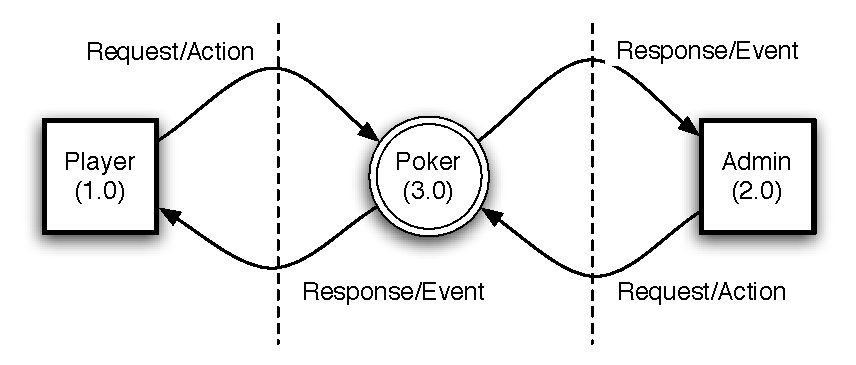
\includegraphics[scale=0.8]{context_diagram}
  \end{center}
  \caption{Context Level DFD}\label{fig:context}
\end{figure}

\begin{figure}[htpb]
  \begin{center}
    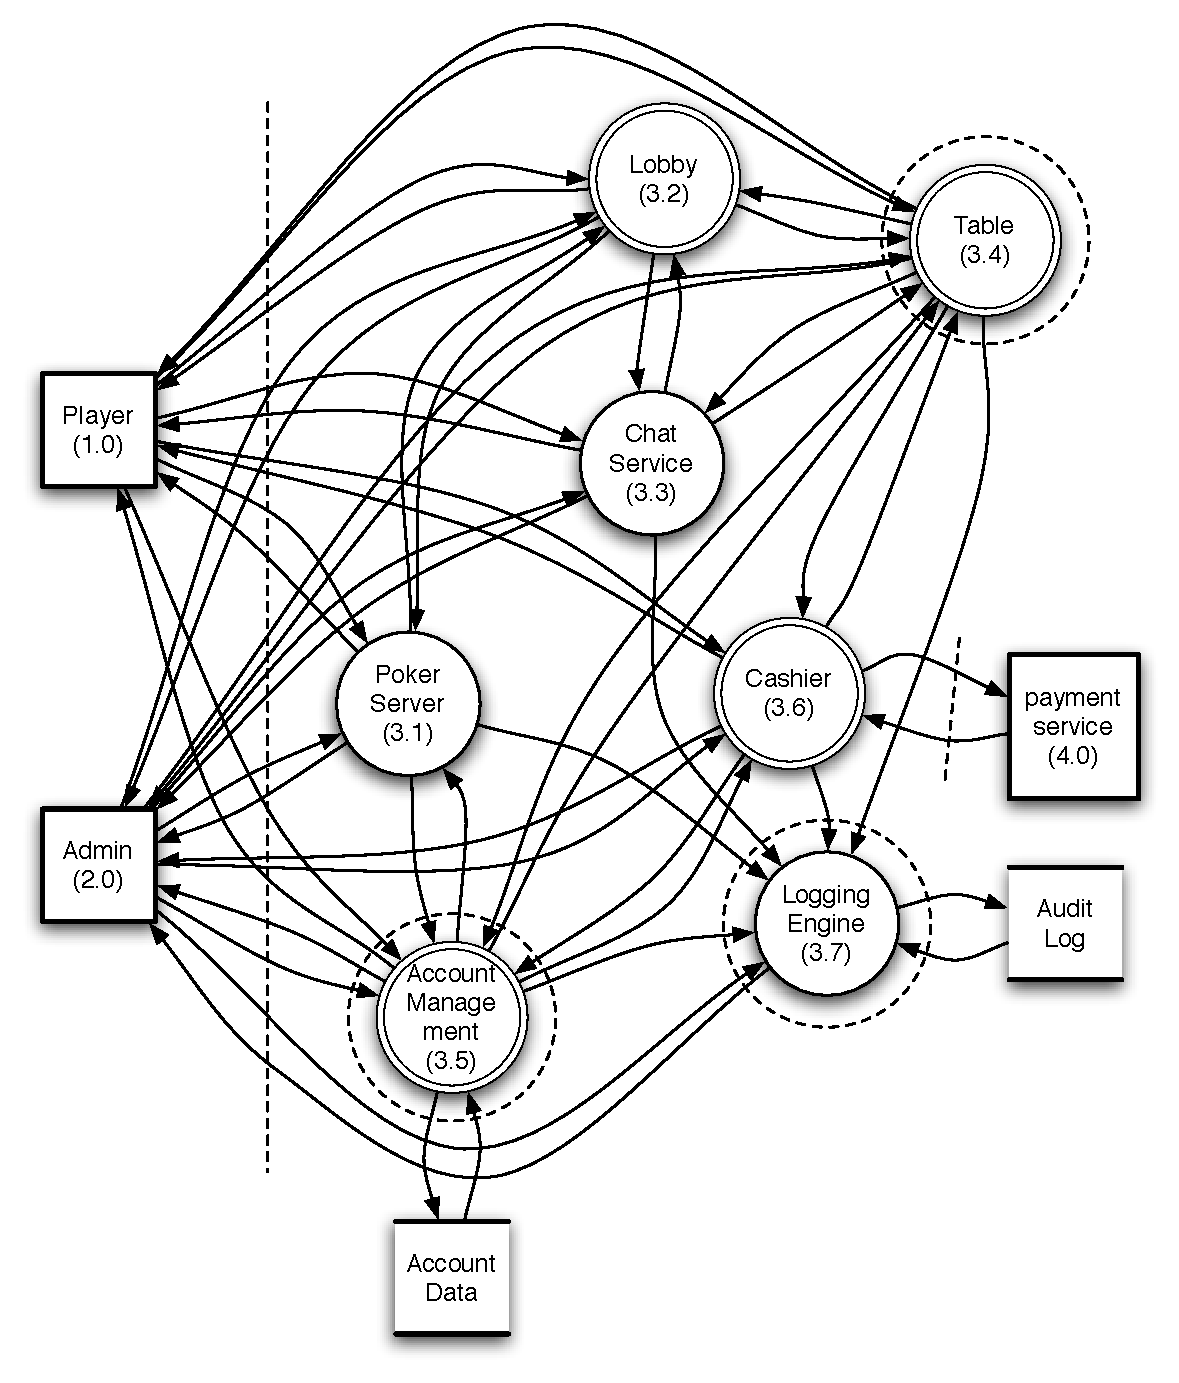
\includegraphics[scale=0.8]{dfd_level_0}
  \end{center}
  \caption{DFD Level-0}\label{fig:level_0}
\end{figure}

\begin{figure}[htpb]
  \begin{center}
    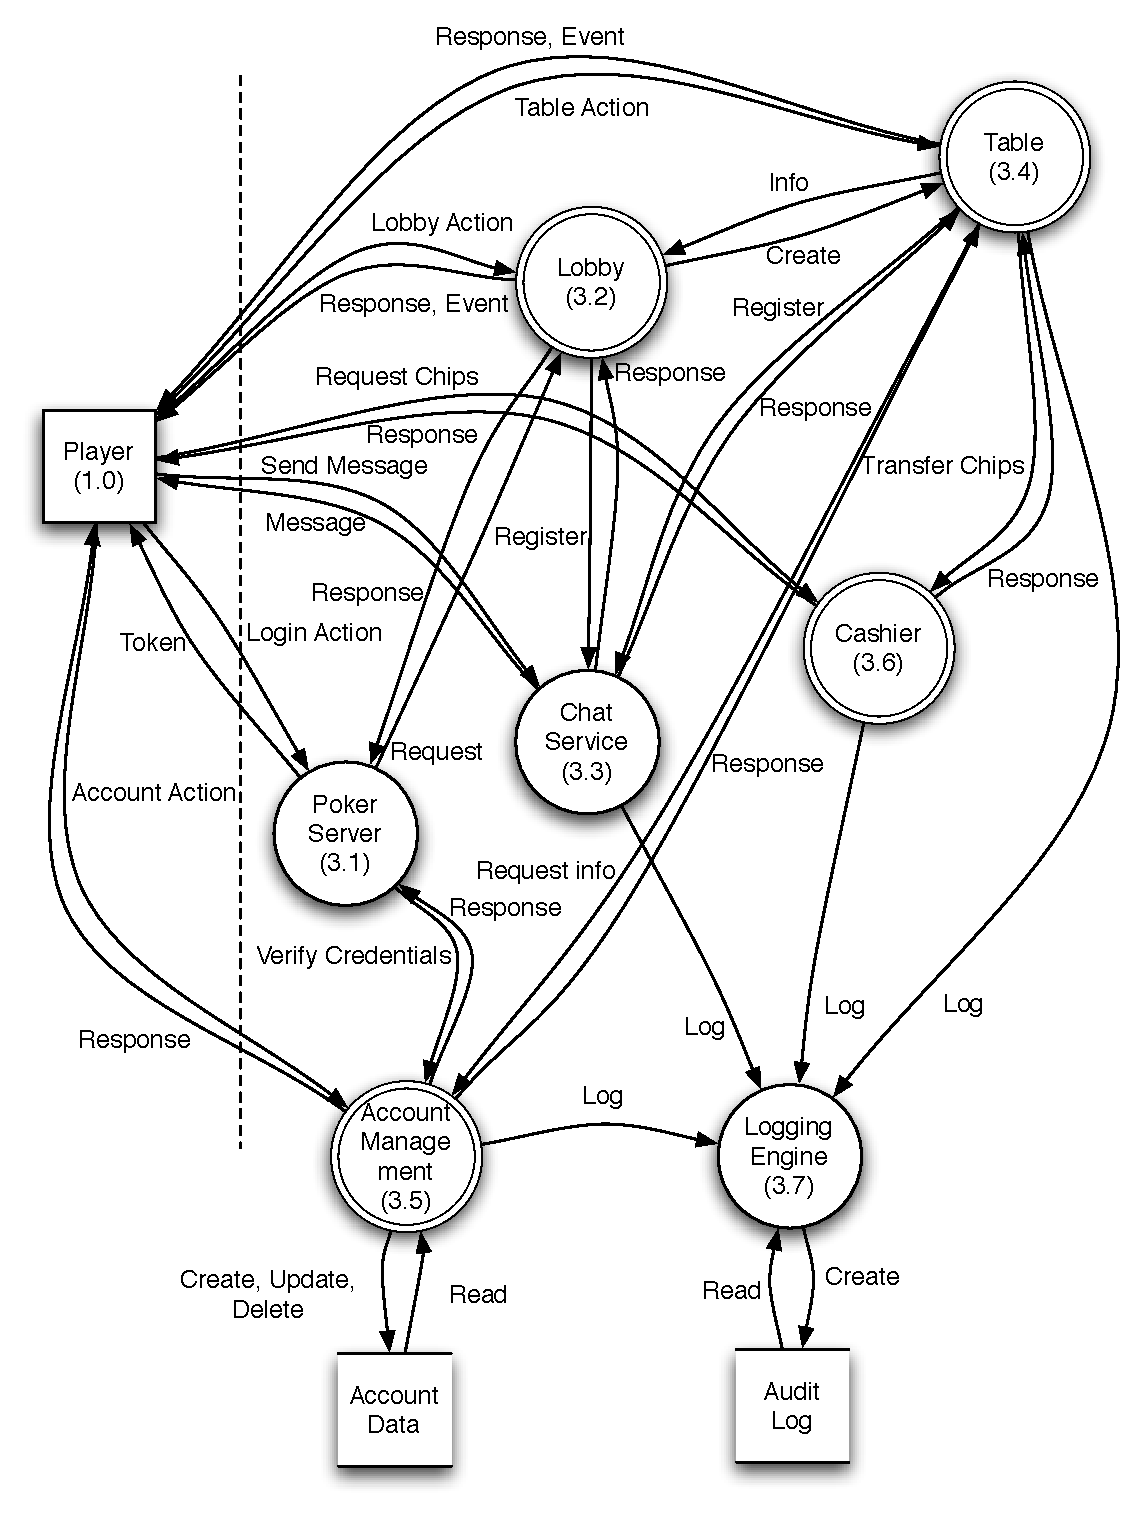
\includegraphics[scale=0.7]{dfd_level_0_player}
  \end{center}
  \caption{DFD Level-0 - only player}\label{fig:level_0_player}
\end{figure}

\section{Rationale}

\subsection{Assumptions}
Some plausible assumptions can simplify the future analysis:
\begin{itemize}
\item There is an internal policy to restrict physical access to the servers.
\item There is no protection needed against an administrator with a debugger (can read and alter memory).
\item Side channels aren't available to mis-actors.
\item Data flow from a process to a data store is in our case always local and not subject to threats.
\end{itemize}

\subsection{Decisions}

We took some decisions that make the analysis easier:
\begin{itemize}
\item We decided to only consider the RMI protocol as communication protocol for the poker application in this
security analysis and not got into depth in the sockets or HTTP protocol. For these protocols, a front-end is added to the architecture that delegates to the different processes also used by RMI.
\item The Table process communicates with Cashier instead of the Account Management process to move an amount of chips
from the main stack of a player to the table stack of that player.
\item For liability reasons, the log with game details must be made public after a game. This is reflected in some
business threats where a mis-actor might use this to profile certain players.
\item We decided to connect the complex processes in the Level 0 DFD directly to the data stores so we can apply STRIDE
at this level. Otherwise the number of misuse cases would explode.
\end{itemize}

\section{Mapping STRIDE to DFD elements}

Taking the elements in figure \ref{fig:level_0} and mapping the STRIDE threats to them results in the following table. The external entities \textit{Admin} and \textit{Payment Service} are subject to a number of threats that we chose not to go into detail for. Data flows from and to these entities are also not considered here. Similarly, data flows from and to the data stores are omitted.

\vspace{0.3cm}
\begin{center}
\begin{tabular}{| c || c || c | c | c | c | c | c |}
  \hline
  \textbf{DFD Element} 	& \textbf{Section}		& \textbf{S} 	& \textbf{T} 	& \textbf{R} 	& \textbf{I} 	& \textbf{D} 	& \textbf{E}	\\\hline
  \hline
  Player 		& \ref{PlayerCases}		& \ref{PlayerCasesS} 	& 	& \ref{PlayerCasesR} 		&  		&  		& 		\\\hline
  Admin 		& /			& / 		& 		& / 		&  		&  		& 		\\\hline
  Payment Service 	& /			& / 		& 		& / 		&  		&  		& 		\\\hline
  \hline
  Poker Server 		& \ref{PokerServerCases}	& \ref{PokerServerCasesS} 	& \ref{PokerServerCasesT}	& \ref{PokerServerCasesR} 	& \ref{PokerServerCasesI} 	& \ref{PokerServerCasesD} 	& \ref{PokerServerCasesE}	\\\hline
  Lobby 		& \ref{LobbyCases}		& \ref{LobbyCasesS} 	& \ref{LobbyCasesT}	& \ref{LobbyCasesR} 	& \ref{LobbyCasesI} 	& \ref{LobbyCasesD} 	& \ref{LobbyCasesE}	\\\hline
  Table 		& \ref{TableCases}		& \ref{TableCasesS} 	& \ref{TableCasesT}	& \ref{TableCasesR} 	& \ref{TableCasesI} 	& \ref{TableCasesD} 	& \ref{TableCasesE}	\\\hline
  Account Management 	& \ref{AccountManagementCases} 	& \ref{AccountManagementCasesS} 	& \ref{AccountManagementCasesT}	& \ref{AccountManagementCasesR} 	& \ref{AccountManagementCasesI} 	& \ref{AccountManagementCasesD} 	& \ref{AccountManagementCasesE}	\\\hline
  Logging Engine 	& \ref{LoggingEngineCases}	& \ref{LoggingEngineCasesS} 	& \ref{LoggingEngineCasesT}	& \ref{LoggingEngineCasesR} 	& \ref{LoggingEngineCasesI} 	& \ref{LoggingEngineCasesD} 	& \ref{LoggingEngineCasesE}	\\\hline
  Chat Service 		& /			& / 	& /	& / 	& / 	& / 	& /	\\\hline
  Cashier 		& /			& / 	& /	& / 	& / 	& / 	& /	\\\hline
  \hline
  Audit Log 		& \ref{AuditLogCases}		& 	& \ref{AuditLogCasesT}	& \ref{AuditLogCasesR} 	& \ref{AuditLogCasesI} 	& \ref{AuditLogCasesD}	& 	\\\hline
  Account Data 		& \ref{AccountDataCases}	& 	& \ref{AccountDataCasesT}	&  	& \ref{AccountDataCasesI} 	& \ref{AccountDataCasesD}	& 	\\\hline
  \hline
  Player $\leftrightarrow$
  Poker Server 		& \ref{PlayerFlowCases}		&	& \ref{PlayerFlowCasesT1}	&	& \ref{PlayerFlowCasesI1}	& \ref{PlayerFlowCasesD1}	&\\
  $\vdots$		& 				&	& \ref{PlayerFlowCasesT2}	&	& \ref{PlayerFlowCasesI2}	& \ref{PlayerFlowCasesD2}	&	\\
  			&				&	& \ref{PlayerFlowCasesT3}	&	& \ref{PlayerFlowCasesI3}	& \ref{PlayerFlowCasesD3}	\\
  			&				&	& \ref{PlayerFlowCasesT4}	&	& \ref{PlayerFlowCasesI4}	& \ref{PlayerFlowCasesD4}	\\\hline
  Table $\leftrightarrow$
  Logging Engine 	& \ref{LoggingEngineFlowCases}	&	& \ref{LoggingEngineFlowCasesT}	&	& \ref{LoggingEngineFlowCasesI}	& \ref{LoggingEngineFlowCasesD}	&	\\
  $\vdots$		& 				&	& 	&	& 	& 	&	\\\hline
\end{tabular}
\end{center}
\vspace{0.3cm}

For the remaining data flows we chose to analyse them as a set of 4 different abstractions. Section \ref{PlayerFlowCases} goes into more detail.

Furthermore, the processes \textit{Chat Service} and \textit{Cashier} are not elaborated on because they are more independent of other processes and functionality.

\section{Architecture based Misuse Cases}
\label{MisUseCases}

The misuse cases are ordered by the entity under threat. Not all threats are equally important though. Repudiation is an important threat with legal consequences. Information disclosure is also important because it makes cheating very easy. Denial of Service attacks are less profitable for crooks and therefore less likely.

Threats that are located more to the exterior of te system (closer to the Player) are more likely to be feasible and are more important. For this reason we completely specified the threats for the Player and Poker Server. Because there are many data flows, we chose to completely specify the threats for the different abstractions in section \ref{PlayerFlowCases} and \ref{LoggingEngineFlowCases}. Between the two data stores we chose to go in to detail for the account data in order to cover all the different element types in the analysis.

\subsection{Player}
\label{PlayerCases}
\subsubsection{Spoofing a Player}
\label{PlayerCasesS}
\textbf{Summary:} \\
The mis-actor gains access to the poker server pretending to be a legitimate user. To achieve this goal he can use false credentials or credentials of an existing user. He could also bypass the authentication system to realize the same objective. \\
\textbf{Primary mis-actor:}
\begin{itemize}
\item Crook
\end{itemize}
\textbf{Basic path:}
\begin{itemize}
\item The mis-actor finds a way to fake credentials.
\item The mis-actor authenticates with the poker server with those fake credentials.
\end{itemize}
\textbf{Alternative paths:}
\begin{itemize}
\item The mis-actor bypasses the authentication system by exploiting a weakness.
\item The mis-actor obtains the credentials of a legitimate player.
\end{itemize}
\textbf{Capture points:}
\begin{itemize}
\item \textbf{Prevention:}
\begin{itemize}

\item Make sure credentials are well protected on the server side.
\item Transmit credentials over the wire securely.
\item Test credentials for uniqueness and complexity.
\item Certify client software to enforce that credentials are handled securely.
\end{itemize}
\end{itemize}
\textbf{Triggers:}\\
Always true, i.e., this can happen at any time. \\
\textbf{Preconditions:}
\begin{itemize}
\item Credentials can be falsified.
\item Credentials are not well protected.
\item There is no authentication system or the authentication system is too weak.
\end{itemize}
\textbf{Assumptions:}
\begin{itemize}
\item The players are careless with their credentials (e.g. store user name/password in a text file).
\item The players choose easy passwords.
\end{itemize}
\textbf{Worst case threat:}\\
The crook can play with the spoofed identity against his own identity and win all chips from spoofed identity. \\
\textbf{Prevention Guarantee:} \\
Only authentic users can gain access at the poker server. \\
\textbf{Stakeholders and risks:}
\begin{itemize}
\item Player:
\begin{itemize}
\item Potential loss of money if his identity is misused and all chips are transfered to an other account.
\end{itemize}
\item Online Casino:
\begin{itemize}
\item Lost confidence if security problems get publicized.
\end{itemize}
\end{itemize}

\subsubsection{Repudiation of a Player}
\label{PlayerCasesR}
\label{Repudiation of a Player}
\textbf{Primary mis-actor:}
\begin{itemize}
\item Crook
\end{itemize}
\textbf{Basic path:}
\begin{itemize}
\item The mis-actor performs an action or transaction.
\item The mis-actor repudiates the action or transaction. For example, he repudiates his bet when it turns out that another player has a better hand.
\item The system fails to prove that the mis-actor is responsible because there is no log or the log is not reliable.
\end{itemize}
\textbf{Alternative paths:}
\begin{itemize}
\item The mis-actor tampers with the logging process to remove evidence.
\end{itemize}
\textbf{Capture points:}
\begin{itemize}
\item \textbf{Prevention:}
\begin{itemize}
\item Use a strong signature system for messages originating from the player.
\item Use antireplay defences.
\item Securely log all actions and transactions. This logged data is trusted to be real and serves as proof.
\item Secure access to the logging process.
\end{itemize}
\end{itemize}

\subsection{Poker Server}
\label{PokerServerCases}
\subsubsection{Spoofing the poker server}
\label{PokerServerCasesS}
\textbf{Primary mis-actor:}
\begin{itemize}
\item Crook
\end{itemize}
\textbf{Basic path:}
\begin{itemize}
\item The mis-actor prepares the process that can spoof a poker server.
\item The mis-actor deploys its process on the online casino servers (performed by a skilled insider).
\end{itemize}
\textbf{Alternative paths:}
\begin{itemize}
\item The mis-actor deploys its process on an external server (performed by a skilled outsider).
\end{itemize}
\textbf{Capture points:}
\begin{itemize}
\item \textbf{Prevention:}
\begin{itemize}
\item Only administrators of the online casino can place code on the online poker servers.
\item Only the code that is running on trusted locations can be used as part of the system.
\item Poker servers are authenticated.
\item Messages coming out of the poker server are signed.
\end{itemize}
\end{itemize}

\subsubsection{Tampering with the poker server}
\label{PokerServerCasesT}
\textbf{Primary mis-actor:}
\begin{itemize}
\item Crook
\end{itemize}
\textbf{Basic path:}
\begin{itemize}
\item The mis-actor sends invalid input to the poker server.
\item The message corrupts the state of the poker server.
\item While the poker server is in the corrupted state, the mis-actor controls the behavior of that poker server.
\item The mis-actor can cheat by changing the behaviour of the poker server.
\end{itemize}
\textbf{Alternative paths:}
\begin{itemize}
\item The mis-actor provides false credentials (spoofing an administrator) and modifies the poker server.
\end{itemize}
\textbf{Capture points:}
\begin{itemize}
\item \textbf{Prevention:}
\begin{itemize}
\item All input is validated.
\item Spoofing an administrator should be impossible.
\end{itemize}
\end{itemize}

\subsubsection{Repudiation of the poker server}
\label{PokerServerCasesR}
\textbf{Primary mis-actor:}
\begin{itemize}
\item Malicious Online Casino Admin
\end{itemize}
\textbf{Basic path:}
\begin{itemize}
\item The mis-actor gains access to the poker server.
\item The mis-actor sends back a response to the player that is misleading (such as incorrect cards).
\item The mis-actor repudiates having sent the response in question.
\item The player fails to prove that the server/mis-actor is responsible because there is no log or the log is not reliable.
\end{itemize}
\textbf{Alternative paths:}
\begin{itemize}
\item The mis-actor tampers with the logging process to remove evidence.
\end{itemize}
\textbf{Capture points:}
\begin{itemize}
\item \textbf{Prevention:}
\begin{itemize}
\item Use a strong signature system for messages sent to the player.
\item Use antireplay defences.
\item Securely log all actions and transactions.
\item Secure access to the logging process.
\end{itemize}
\end{itemize}

\subsubsection{Information disclosure at the poker server}
\label{PokerServerCasesI}
\textbf{Primary mis-actor:}
\begin{itemize}
\item Crook
\end{itemize}
\textbf{Basic path:}
\begin{itemize}
\item The mis-actor spoofs another actor with access to private information (e.g. user names, passwords, ...).
\item The mis-actor uses the private information.
\end{itemize}
\textbf{Alternative paths:}
\begin{itemize}
\item Elevation of privilege of the mis-actor leads to information disclosure.
\item The mis-actor sends invalid input to the poker server.
\end{itemize}
\textbf{Capture points:}
\begin{itemize}
\item \textbf{Prevention:}
\begin{itemize}
\item All input is validated.
\end{itemize}
\end{itemize}

\subsubsection{DoS against the poker server}
\label{PokerServerCasesD}
\textbf{Primary mis-actor:}
\begin{itemize}
\item Crook
\end{itemize}
\textbf{Basic path:}
\begin{itemize}
\item The mis-actor sends invalid input to the poker server.
\item The poker server crashes.
\item The poker server becomes unavailable.
\end{itemize}
\textbf{Alternative paths:}
\begin{itemize}
\item The mis-actor crashes the poker server by tampering with the poker server.
\item The mis-actor consumes application-specific resources (e.g. send more login requests per second than the poker server can handle).
\item The mis-actor consumes fundamental resources.
\end{itemize}
\textbf{Capture points:}
\begin{itemize}
\item \textbf{Prevention:}
\begin{itemize}
\item All input is validated.
\item The poker server is load-balanced.
\end{itemize}
\item \textbf{Detection:}
\begin{itemize}
\item Access to the poker server is securely logged.
\end{itemize}
\end{itemize}

\subsubsection{Elevation of privilege at the poker server}
\label{PokerServerCasesE}
\textbf{Primary mis-actor:}
\begin{itemize}
\item Crook
\end{itemize}
\textbf{Basic path:}
\begin{itemize}
\item The mis-actor logs in.
\item He activates the role (administrator) with higher privileges.
\item The mis-actor gains higher privileges.
\item The mis-actor misuses the higher privileges.
\end{itemize}
\textbf{Alternative paths:}
\begin{itemize}
\item The mis-actor spoofs the identity of an other actor (administrator) with higher privileges.
\item The mis-actor tampers with the poker server to gain more privileges.
\item The mis-actor sends invalid input to the poker server.
\end{itemize}
\textbf{Capture points:}
\begin{itemize}
\item \textbf{Prevention:}
\begin{itemize}
\item Authentication and authorization system that verifies credentials.
\item Spoofing user and tampering with poker server prevention.
\end{itemize}
\item \textbf{Detection:}
\begin{itemize}
\item Access to the poker server is securely logged. The log can be compared with the security policy to verify if an actor is allowed to do the action.
\end{itemize}
\end{itemize}

\subsection{Lobby}
\label{LobbyCases}
\subsubsection{Spoofing a lobby}
\label{LobbyCasesS}
\textbf{Summary:} \\
The mis-actor prepares a process to spoof the lobby and deploys it on one of the online casino servers or on an external server. Players can be tricked into connecting with the spoofed lobby.
\subsubsection{Tampering with the lobby}
\label{LobbyCasesT}
\textbf{Summary:} \\
The mis-actor tampers with the lobby to modify its functionality. A player connecting to a table through the lobby can be diverted to an untrusted table.
\subsubsection{Repudiation of an action at the lobby}
\label{LobbyCasesR}
\textbf{Summary:} \\
The lobby can deny access to a table for a certain user and deny having done so.

\subsubsection{Information disclosure at the lobby}
\label{LobbyCasesI}
\textbf{Summary:} \\
The mis-actor can obtain private information through spoofing or tampering with the lobby process. He could see private tables or tournament settings.

\subsubsection{DoS against the lobby}
\label{LobbyCasesD}
\textbf{Summary:} \\
The mis-actor performs actions leading to a crash or overloading the capacity of the lobby. As a result, the lobby can no longer be reached by the users.

\subsubsection{Elevation of privilege at the lobby}
\label{LobbyCasesE}
\textbf{Summary:} \\
The mis-actor can do administrator actions. He can achieve this by presenting false credentials, spoofing an administrator or tampering with the lobby or account management.

\subsection{Table}\
\label{TableCases}
\subsubsection{Spoofing a table}
\label{TableCasesS}
\textbf{Summary:} \\
The mis-actor prepares a process to spoof the table and deploys it on one of the online casino servers or on an external server. Every player connecting to this table can be scammed.
\subsubsection{Tampering with a table}
\label{TableCasesT}
\textbf{Summary:} \\
The mis-actor tampers with the table to modify its functionality. Every player connecting to this table can be scammed. The tampered table could provide the mis-actor with confidential information or deal crafted hands to maximize the profit of the mis-actor (e.g. deal a full house to an innocent player and deal a four of a kind to himself and lure the innocent player to go all-in).
\subsubsection{Repudiation of an action at a table}
\label{TableCasesR}
\textbf{Summary:} \\
The online casino denies that a player has won a number of chips or has received certain hole cards. This is possible if there is no log or if the log could be modified. It is also possible that the hand evaluation system has been tampered with. This should be detected afterwards.
\subsubsection{Information disclosure at a table}
\label{TableCasesI}
\textbf{Primary mis-actor:}
\begin{itemize}
\item Crook
\end{itemize}
\textbf{Basic path:}
\begin{itemize}
\item The mis-actor spoofs an other actor with access to private information regarding this table
(e.g. pocket cards of players, ...).
\item The mis-actor uses the private information.
\end{itemize}
\textbf{Alternative paths:}
\begin{itemize}
\item Elevation of privilege of the mis-actor leads to information disclosure.
\item The mis-actor sends invalid input to the table.
\end{itemize}
\textbf{Capture points:}
\begin{itemize}
\item \textbf{Prevention:}
\begin{itemize}
\item All input is validated.
\end{itemize}
\item \textbf{Detection:}
\begin{itemize}
\item The behavior of the mis-actor is influenced by the information disclosure. This altered behavior could be detected by examining the logs for statistical anomalies.
\end{itemize}
\end{itemize}

\subsubsection{DoS against a table}
\label{TableCasesD}
\textbf{Summary:} \\
The mis-actor performs actions leading to a crash or overloading the capacity of the table. As a result, the table can no longer be reached by the users.

\subsubsection{Elevation of Privilege at the table}
\label{TableCasesE}
\textbf{Summary:} \\
The mis-actor can do administrator actions. He can achieve this by presenting false credentials, spoofing an administrator or tampering with the table or account management.

\subsection{Account Management}
\label{AccountManagementCases}

\subsubsection{Spoofing the account management system}
\label{AccountManagementCasesS}
\textbf{Summary:} \\
The mis-actor gains access to the account management server or manages to pretend he is the account management system by obtaining or falsifying credentials. By doing so, the mis-actor can trick other processes into thinking they're dealing with the real account management system.

\subsubsection{Tampering with the account management system}
\label{AccountManagementCasesT}
\textbf{Summary:} \\
The mis-actor can tamper with the account management system to always accept credentials for a certain fake user.

\subsubsection{Repudiation of using the account management system}
\label{AccountManagementCasesR}
\textbf{Summary:} \\
The casino can deny access to a user in critical moments and deny having done so. When a user changes his credit card number or other personal information the account management system can deny having received that request. When a payment fails afterwards the user cannot seek compensation from the casino.

\subsubsection{Information disclosure of the account management system}
\label{AccountManagementCasesI}
\textbf{Summary:} \\
When the mis-actor compromises the account management system, he can obtain private information such as passwords and credit card numbers. This can be done by spoofing or tampering with the process.

\subsubsection{DoS against the account management system}
\label{AccountManagementCasesD}
\textbf{Summary:} \\
By sending bad input to the account management system or by sending many requests at once, the mis-user can overload the process. This can result in legitimate users not being able to authenticate with the system or change their account data.

\subsubsection{Elevation of Privilege at the account management system}
\label{AccountManagementCasesE}
\textbf{Summary:} \\
Through spoofing, tampering or exploiting the authorization system, the mis-actor can obtain admin privileges. In the account management system he will be able to e.g. kick or ban opponents.

\subsection{Logging Engine}
\label{LoggingEngineCases}

\subsubsection{Spoofing the logging engine}
\label{LoggingEngineCasesS}
\textbf{Summary:} \\
The mis-actor gains access to the logging server or manages to pretend to be the logging engine by obtaining or falsifying credentials. This way other processes can be tricked into sending their logging data to the spoofed process.

\subsubsection{Tampering with the logging engine}
\label{LoggingEngineCasesT}
\textbf{Summary:} \\
The mis-actor can tamper with the logging engine and send different data to the audit log than was received from other processes. Alternatively, he can send logging data to the audit log that is made up.

\subsubsection{Repudiation of using the logging engine}
\label{LoggingEngineCasesR}
\textbf{Summary:} \\
The logging engine can deny having recieved logging data that didn't make it to the physical audit log. The casino can deny that certain valid audit data was sent from the logging engine.

\subsubsection{Information disclosure of the logging engine}
\label{LoggingEngineCasesI}
\textbf{Summary:} \\
The mis-actor can obtain private information through spoofing or tampering with the logging process. This way he could e.g. see the hidden cards of an opponent when they are being logged.

\subsubsection{DoS against the logging engine}
\label{LoggingEngineCasesD}
\textbf{Summary:} \\
By sending bad data to the logging engine or by sending many requests at once, the mis-user can overload the process. This can result in valid logging data being lost by the process because it can't store the incoming information.

\subsubsection{Elevation of Privilege at the logging engine}
\label{LoggingEngineCasesE}
\textbf{Summary:} \\
Through spoofing, tampering or exploiting the authorization system, the mis-actor can obtain admin privileges. As a result he can, for instance, shut down logging.

\subsection{Audit Log}
\label{AuditLogCases}

\subsubsection{Tampering with the audit log}
\label{AuditLogCasesT}
\textbf{Summary:} \\
The misuser can tamper with the audit log when he bypasses the protection or monitor, or when he exploits overcapacity failures. The logging data can then be modified or erased.

\subsubsection{Repudiation of logging something in the audit log}
\label{AuditLogCasesR}
\textbf{Summary:} \\
The mis-actor can modify or obscure data in the audit log to be able to
repudate certain actions. An auditor will not be able to deny this
allegation.

Also see section \ref{Criticism}, ``Repudiaton of processes/data stores'', for criticism of this threat.

\subsubsection{Information disclosure of the audit log}
\label{AuditLogCasesI}
\textbf{Summary:} \\
When the mis-actor bypasses the protection scheme and the data is weakly encrypted he might be able to obtain logging information. This can e.g be credit card information, transaction information or private cards. Information leakage can also occur when removed data isn't cleared correctly from the data store or when the mis-actor spoofs an entity that has access to the data store.

\subsubsection{DoS against the audit log}
\label{AuditLogCasesD}
\textbf{Summary:} \\
By sending bad data to the audit log (e.g. SQL injecton) or by sending many requests at once, the mis-user can overload the data store. This can result in valid logging data being lost because the data store has run out of memory or disk space.

\subsection{Account Data}
\label{AccountDataCases}

\subsubsection{Tampering with account data}
\label{AccountDataCasesT}
\textbf{Primary mis-actor:}
\begin{itemize}
\item Crook
\end{itemize}
\textbf{Basic path:}
\begin{itemize}
\item The mis-actor gains access to the data store
\item The mis-actor puts data directly into the data store
\end{itemize}
\textbf{Alternative paths:}
\begin{itemize}
\item The mis-actor removes data directly from the data store
\item There may be overcapacity failures: the mis-actor floods the data store by placing large
amounts of data into the data store. As a consequence data in the beginning of the store might be overwritten, data written to the store might be discarded or the data store might crash depending on the implementation of
the data store.
\end{itemize}
\textbf{Capture points:}
\begin{itemize}
\item \textbf{Prevention:}
\begin{itemize}
\item Adding and removing data in the data store is securely logged.
\item The data store is protected by the internal policies.
\item Extra-monitor access is impossible (behind a reliable firewall).
\item Overcapacity failures are handled correctly.
\item Only private or local networks are used for communication between the account management process
and the account data store.
\end{itemize}
\item \textbf{Detection:}
\begin{itemize}
\item The logs can be searched for add or remove operations.
\end{itemize}
\end{itemize}

\subsubsection{Information disclosure of account data}
\label{AccountDataCasesI}
\textbf{Primary mis-actor:}
\begin{itemize}
\item Crook
\end{itemize}
\textbf{Basic path:}
\begin{itemize}
\item The mis-actor gains access to the data store.
\item The mis-actor reads private data from data store.
\end{itemize}
\textbf{Alternative paths:}
\begin{itemize}
\item The mis-actor spoofs the account management process
\end{itemize}
\textbf{Capture points:}
\begin{itemize}
\item \textbf{Prevention:}
\begin{itemize}
\item Encrypting the data
\item The data store is protected by the internal policies.
\item Extra-monitor access is impossible (behind a reliable firewall).
\item Only private or local networks are used for communication between the account management process
and the account data store.
\item Prevent spoofing of the account management process.
\end{itemize}
\end{itemize}

\subsubsection{DoS against account data}
\label{AccountDataCasesD}
\textbf{Primary mis-actor:}
\begin{itemize}
\item Crook
\end{itemize}
\textbf{Basic path:}
\begin{itemize}
\item The mis-actor gains access to the data store.
\item The mis-actor corrupts the data store by sending invalid input.
\item The data store crashes and becomes unavailable.
\end{itemize}
\textbf{Alternative paths:}
\begin{itemize}
\item The mis-actor floods the data store by placing large amounts of data into the data store, exceeding its capacity.
\item The mis-actor consumes application-specific resources (e.g. submit more queries per second that the data
store can handle).
\item The mis-actor injects malicious SQL queries (or others) into a process that uses the data store. When this injection reaches the data store it crashes.
\end{itemize}
\textbf{Capture points:}
\begin{itemize}
\item \textbf{Prevention:}
\begin{itemize}
\item Invalid queries are filtered.
\item The data store is protected by the internal policies.
\item Extra-monitor access is impossible (behind a reliable firewall).
\item Only private or local networks are used for communication between the account management process
and the account data store.
\item The data store is load-balanced.
\end{itemize}
\end{itemize}

\subsection{Data Flows from a Player}
\label{PlayerFlowCases}

According to \cite[p117]{1202957}, one of the first concerns before doing threat analysis should be to reduce the number of entities to analyze.
Here we choose to reduce the number of data flows from/to the Player because interaction between a Player and the different processes is very similar (using the same technology, similar entities with similar confidentiality). We only consider requests for tokens (login actions), actions sent to a process, tokens sent to a Player and events/responses sent to a Player.

\subsubsection{Tampering with token requests}
\label{PlayerFlowCasesT1}
\textbf{Primary mis-actor:}
\begin{itemize}
\item Crook
\end{itemize}
\textbf{Basic path:}
\begin{itemize}
\item The mis-actor intercepts a token request sent by another Player.
\item The mis-actor replays the token request to obtain a token.
\end{itemize}
\textbf{Alternative paths:}
\begin{itemize}
\item The mis-actor spoofs another Player to send fake token requests.
\item The mis-actor performs a MITM attack\footnote{Man-in-the-middle attack} and eavesdrops on the token requests sent by a genuine Player.
\end{itemize}
\textbf{Capture points:}
\begin{itemize}
\item \textbf{Prevention:}
\begin{itemize}
\item Use antireplay defences and a strong message and channel integrity algorithm.
\item Prevent spoofing of Players.
\end{itemize}
\end{itemize}

\subsubsection{Tampering with tokens}
\label{PlayerFlowCasesT2}
\textbf{Primary mis-actor:}
\begin{itemize}
\item Crook
\end{itemize}
\textbf{Basic path:}
\begin{itemize}
\item The mis-actor intercepts a token.
\item The mis-actor modifies a token before sending it to the Player in a MITM attack. The modified token can refer to a process spoofed by the mis-actor.
\end{itemize}
\textbf{Alternative paths:}
\begin{itemize}
\item The mis-actor spoofs the Poker Server to send fake tokens.
\item The mis-actor replays tokens.
\end{itemize}
\textbf{Capture points:}
\begin{itemize}
\item \textbf{Prevention:}
\begin{itemize}
\item Use antireplay defences and a strong message and channel integrity algorithm.
\item Prevent spoofing of the Poker Server.
\end{itemize}
\end{itemize}

\subsubsection{Tampering with actions}
\label{PlayerFlowCasesT3}
\textbf{Primary mis-actor:}
\begin{itemize}
\item Crook
\end{itemize}
\textbf{Basic path:}
\begin{itemize}
\item The mis-actor changes messages to his advantage, sends fake messages that go undetected or replays messages sent by a Player. For example, the mis-actor can replace the bet amount by a larger number when he has very good cards)
\end{itemize}
\textbf{Alternative paths:}
\begin{itemize}
\item The mis-actor violates the integrity of the channel to tamper with the data flow.
\item The mis-actor spoofs a Player to send fake actions.
\end{itemize}
\textbf{Capture points:}
\begin{itemize}
\item \textbf{Prevention:}
\begin{itemize}
\item Use antireplay defences and a strong message and channel integrity algorithm.
\item Prevent spoofing of Players.
\end{itemize}
\end{itemize}

\subsubsection{Tampering with responses and events}
\label{PlayerFlowCasesT4}
\textbf{Primary mis-actor:}
\begin{itemize}
\item Crook
\end{itemize}
\textbf{Basic path:}
\begin{itemize}
\item The mis-actor changes events to his advantage, sends fake events or replays events For example, the mis-actor can replace the pocket cards sent to another player by aces to trick him into betting excessively.
\end{itemize}
\textbf{Alternative paths:}
\begin{itemize}
\item The mis-actor violates the integrity of the channel to tamper with the data flow.
\item The mis-actor spoofs the Poker Server to send fake actions.
\end{itemize}
\textbf{Capture points:}
\begin{itemize}
\item \textbf{Prevention:}
\begin{itemize}
\item Use antireplay defences and a strong message and channel integrity algorithm.
\item Prevent spoofing the Poker Server.
\end{itemize}
\end{itemize}


\subsubsection{Information Disclosure of token requests}
\label{PlayerFlowCasesI1}
\textbf{Primary mis-actor:}
\begin{itemize}
\item Crook
\end{itemize}
\textbf{Basic path:}
\begin{itemize}
\item The mis-actor finds a weakness in the confidentiality of token requests and the channel used to send them.
\item The mis-actor observes who is playing and what modules they are requesting tokens for.
\end{itemize}
\textbf{Alternative paths:}
\begin{itemize}
\item The mis-actor sets up a MITM attack.
\end{itemize}
\textbf{Capture points:}
\begin{itemize}
\item \textbf{Prevention:}
\begin{itemize}
\item Use stong message confidentiality.
\item Use strong channel confidentiality.
\end{itemize}
\end{itemize}

\subsubsection{Information Disclosure of tokens}
\label{PlayerFlowCasesI2}
\textbf{Primary mis-actor:}
\begin{itemize}
\item Crook
\end{itemize}
\textbf{Basic path:}
\begin{itemize}
\item The mis-actor finds a weakness in the confidentiality of token message and the channel used to send them.
\item The mis-actor observes the tokens issued to the Player.
\end{itemize}
\textbf{Alternative paths:}
\begin{itemize}
\item The mis-actor sets up a MITM attack.
\end{itemize}
\textbf{Capture points:}
\begin{itemize}
\item \textbf{Prevention:}
\begin{itemize}
\item Use stong message confidentiality.
\item Use strong channel confidentiality.
\end{itemize}
\end{itemize}

\subsubsection{Information Disclosure of actions}
\label{PlayerFlowCasesI3}
\textbf{Primary mis-actor:}
\begin{itemize}
\item Crook
\end{itemize}
\textbf{Basic path:}
\begin{itemize}
\item The mis-actor finds a weakness in the confidentiality of actions and the channel used to send them.
\item The mis-actor observes the actions and can abuse private chat information and other confidential actions performed by the Player.
\end{itemize}
\textbf{Alternative paths:}
\begin{itemize}
\item The mis-actor sets up a MITM attack.
\end{itemize}
\textbf{Capture points:}
\begin{itemize}
\item \textbf{Prevention:}
\begin{itemize}
\item Use stong message confidentiality.
\item Use strong channel confidentiality.
\end{itemize}
\end{itemize}

\subsubsection{Information Disclosure of responses and events}
\label{PlayerFlowCasesI4}
\textbf{Primary mis-actor:}
\begin{itemize}
\item Crook
\end{itemize}
\textbf{Basic path:}
\begin{itemize}
\item The mis-actor finds a weakness in the confidentiality of events/responses and the channel used to send them.
\item The mis-actor observes events that give him an unfair advantage in the game, like the pocket cards of competitors.
\end{itemize}
\textbf{Alternative paths:}
\begin{itemize}
\item The mis-actor sets up a MITM attack.
\end{itemize}
\textbf{Capture points:}
\begin{itemize}
\item \textbf{Prevention:}
\begin{itemize}
\item Use stong message confidentiality.
\item Use strong channel confidentiality.
\end{itemize}
\end{itemize}


\subsubsection{Denial of Service of token requests}
\label{PlayerFlowCasesD1}
\textbf{Primary mis-actor:}
\begin{itemize}
\item Crook
\end{itemize}
\textbf{Basic path:}
\begin{itemize}
\item The mis-actor incapacitates the channel by incapacitating the Player or process.
\item The Player cannot request tokens.
\end{itemize}
\textbf{Alternative paths:}
\begin{itemize}
\item The mis-actor consumes resources required by the Player or process.
\item The mis-actor corrupts the token requests.
\item The mis-actor pre-plays token requests, making that functionality unavailable for a Player.
\end{itemize}
\textbf{Capture points:}
\begin{itemize}
\item \textbf{Prevention:}
\begin{itemize}
\item Prevent tampering, spoofing and DOS of the endpoints and data flow.
\item Limit the number of resources the process depends on.
\end{itemize}
\end{itemize}

\subsubsection{Denial of Service of tokens}
\label{PlayerFlowCasesD2}
\textbf{Primary mis-actor:}
\begin{itemize}
\item Crook
\end{itemize}
\textbf{Basic path:}
\begin{itemize}
\item The mis-actor incapacitates the channel by incapacitating the Player or process.
\item The Player cannot receive tokens.
\end{itemize}
\textbf{Alternative paths:}
\begin{itemize}
\item The mis-actor consumes resources required by the Player or process.
\end{itemize}
\textbf{Capture points:}
\begin{itemize}
\item \textbf{Prevention:}
\begin{itemize}
\item Prevent tampering, spoofing and DOS of the endpoints and data flow.
\item Limit the number of resources the process depends on.
\end{itemize}
\end{itemize}

\subsubsection{Denial of Service of actions}
\label{PlayerFlowCasesD3}
\textbf{Primary mis-actor:}
\begin{itemize}
\item Crook
\end{itemize}
\textbf{Basic path:}
\begin{itemize}
\item The mis-actor incapacitates the channel by incapacitating the Player or process.
\item The Player cannot perform actions. For example, this can lead to timeouts where the server folds on behalf of a non-responsive player, giving an unfair advantage to the mis-actor.
\end{itemize}
\textbf{Alternative paths:}
\begin{itemize}
\item The mis-actor consumes resources required by the Player or process.
\item The mis-actor corrupts the actions.
\item The mis-actor pre-plays actions, making them unavailable for a Player.
\end{itemize}
\textbf{Capture points:}
\begin{itemize}
\item \textbf{Prevention:}
\begin{itemize}
\item Prevent tampering, spoofing and DOS of the endpoints and data flow.
\item Limit the number of resources the process depends on.
\end{itemize}
\end{itemize}

\subsubsection{Denial of Service of responses and events}
\label{PlayerFlowCasesD4}
\textbf{Primary mis-actor:}
\begin{itemize}
\item Crook
\end{itemize}
\textbf{Basic path:}
\begin{itemize}
\item The mis-actor incapacitates the channel by incapacitating the Player or process.
\item The Player cannot receive events/responses.
\end{itemize}
\textbf{Alternative paths:}
\begin{itemize}
\item The mis-actor consumes resources required by the Player or process.
\end{itemize}
\textbf{Capture points:}
\begin{itemize}
\item \textbf{Prevention:}
\begin{itemize}
\item Prevent tampering, spoofing and DOS of the endpoints and data flow.
\item Limit the number of resources the process depends on.
\end{itemize}
\end{itemize}

\subsection{Data Flows to Logging Engine}
\label{LoggingEngineFlowCases}

\subsubsection{Tampering with logging requests}
\label{LoggingEngineFlowCasesT}
\textbf{Primary mis-actor:}
\begin{itemize}
\item Crook
\end{itemize}
\textbf{Basic path:}
\begin{itemize}
\item The mis-actor intercepts a logging request sent by another process.
\item The mis-actor replays the logging request to duplicate the event to be logged.
\end{itemize}
\textbf{Alternative paths:}
\begin{itemize}
\item The mis-actor spoofs another Player to send fake logging requests.
\item The mis-actor performs a MITM attack and eavesdrop on the logging requests sent by a genuine process.
\end{itemize}
\textbf{Capture points:}
\begin{itemize}
\item \textbf{Prevention:}
\begin{itemize}
\item Use antireplay defences and a strong message and channel integrity algorithm.
\item Prevent spoofing of processes.
\end{itemize}
\end{itemize}

\subsubsection{Information Disclosure of logging requests}
\label{LoggingEngineFlowCasesI}
\textbf{Primary mis-actor:}
\begin{itemize}
\item Crook
\end{itemize}
\textbf{Basic path:}
\begin{itemize}
\item The mis-actor finds a weakness in the confidentiality of logging requests and the channel used to send them.
\item The mis-actor observes which process wants to log something and what they want to log.
\end{itemize}
\textbf{Alternative paths:}
\begin{itemize}
\item The mis-actor sets up a MITM attack.
\end{itemize}
\textbf{Capture points:}
\begin{itemize}
\item \textbf{Prevention:}
\begin{itemize}
\item Use stong message confidentiality.
\item Use strong channel confidentiality.
\end{itemize}
\end{itemize}
\subsubsection{Denial of Service of logging requests}
\label{LoggingEngineFlowCasesD}
\textbf{Primary mis-actor:}
\begin{itemize}
\item Crook
\end{itemize}
\textbf{Basic path:}
\begin{itemize}
\item The mis-actor incapacitates the channel by incapacitating the Logging Engine or the process sending the logging request.
\item Logging is not possible.
\end{itemize}
\textbf{Alternative paths:}
\begin{itemize}
\item The mis-actor consumes resources required by the Logging Engine or the process sending the logging request.
\item The mis-actor corrupts the logging requests.
\item The mis-actor preplays logging requests, making that functionality unavailable for other processes.
\end{itemize}
\textbf{Capture points:}
\begin{itemize}
\item \textbf{Prevention:}
\begin{itemize}
\item Prevent tampering, spoofing and DOS of the endpoints and data flow.
\item Limit the number of resources the process depends on.
\end{itemize}
\end{itemize}

\section{Business Logic Misuse Cases}

\subsection{Single player Cheating}
\subsubsection{A malicious player uses multiple accounts to access more hidden cards}
\textbf{Summary:} \\
The malicious player uses multiple accounts at the same table. He uses the extra information to  have a more accurate view on the outs\footnote{Any unseen card that, if drawn, will improve a player's hand to one that is likely to win. The number of outs can be converted to the probability of making the hand on the next card.}. He gains an unfair advantage over the other innocent players. \\
\textbf{Primary mis-actor:}
\begin{itemize}
\item Crook
\end{itemize}
\textbf{Basic path:}
\begin{itemize}
\item The malicious player creates multiple accounts.
\item The malicious player is sit-in at a table with different accounts.
\item The malicious player uses the additional knowledge to make statistically more successful decisions.
\end{itemize}
\textbf{Capture points:}
\begin{itemize}
\item \textbf{Prevention:}
\begin{itemize}
\item Enforce the policy that each player can have at most one account.
\item Limit the number of simultaneous connections from one IP-address.
\end{itemize}
\item \textbf{Detection:}
\begin{itemize}
\item The behavior of the malicious player is influenced by the extra knowledge. This could lead to inexplicable actions that can only be explained with the knowledge of the pocket cards of the other players. This behavior can be detected by analyzing the logs for statistical anomalies.
\item Detect when two accounts frequently play at the same table.
\end{itemize}
\end{itemize}
\subsubsection{A malicious player with admin rights misuses his privileges}
\textbf{Summary:} If an admin has access to the card information of all the players at a table, he can act on perfect knowledge which is a huge advantage.

\subsubsection{A malicious player misuses the right to ask the admin to view the log of the table}
\textbf{Summary:} \\
The malicious player misuses the possibility to view the table log pretending to be suspicious of collusion. The malicious player can verify the hands of all the opponents, also those who have chosen not to show their cards. This way, he can gain more insight into the strategy of his opponents (whether someone is bluffing or not, ...). If consulting the log is only possible after the game has been played, there is no direct threat but in the long run it gives an unfair advantage and allows profiling of a player's behaviour.

\subsubsection{A malicious player can flood the network of another player to force a time-out}
\textbf{Summary:} \\
A malicious player can flood the network of an opponent at a crucial moment so no communication between this opponent and the poker server is possible. This will lead to a time-out of the opponent. Depending on the time-out policy the malicious player can have a huge advantage.

\subsection{Multiplayer Cheating}
\subsubsection{Collusion}
\textbf{Summary:} \\
Collusion is a secret cooperation of two or more players. By collaborating they have access to more knowledge of hole cards than legitimate players. With this extra knowledge they have a more accurate view on the outs. Another advantage that can be achieved through collaboration is the use of a common strategy to maximise their profits. Examples of strategies are: only playing the best hand they have or raise each other to force the other players to call to enlarge the pot. \\
\textbf{Primary mis-actor:}
\begin{itemize}
\item Unskilled outsiders
\end{itemize}
\textbf{Basic path:}
\begin{enumerate}
\item[bp1.] The mis-actors sit-in at the same table.
\item[bp2.] The mis-actors communicate their hole cards and tactics through some unmonitored channel.
\item[bp3.] The mis-actors take actions with the extra knowledge.
\item[bp4.] The mis-actors gain an unfair advantage over the honest players.
\end{enumerate}
\textbf{Alternative paths:}
\begin{itemize}
\item[ap1.] The mis-actors communicate their hole cards and tactics through a covert channel in a monitored channel. (for bp2.)
\end{itemize}
\textbf{Capture points:}
\begin{itemize}
\item \textbf{Prevention:}
\begin{itemize}
\item All inter player communication happens through a monitored channel where no covert channel is possible. In a monitored channel all messages are accessible to all the players who have joined a table. All the messages are also logged for audit.
\item Enforcing the use of a webcam is an invasive way to mitigate the use of some unmonitored channels (e.g. phone, same physical location, ...), but it's still possible to use parts of the body that aren't captured to send messages to the other mis-actor or to use a covert channel. It's also possible to spoof the stream of the webcam so countermeasures against this new threat have to be taken into account.
\item The screen can be periodically captured and analysed to ensure no other communicative application is used. The applicability of this method lies only in the scope of the computer that is used. This countermeasure is broken by using an other independent computer to communicate with the other mis-actors.
\item A firewall can be placed to disallow all other communication except the poker client, or filter all network packages for suspicious chat messages. This capture point has the same vulnerability as the previous capture point: it's possible to break this countermeasure by using another independent computer to communicate with the other mis-actors.
\end{itemize}
A proper risk analysis is needed to find the right trade-off between cost and risk as absolute mitigation of this threat is practically infeasible.
\item \textbf{Detection:}
\begin{itemize}
\item The game logs are analysed to detect collusion.
\item A player can report suspicious behavior that will be investigated by the online casino.
\end{itemize}
\end{itemize}
\textbf{Triggers:}\\
Always true, i.e., this can happen at any time. \\
\textbf{Preconditions:}
\begin{itemize}
\item The provided chat system is unmonitored.
\item The covert channel is undetectable in a monitored channel.
\end{itemize}
\textbf{Assumptions:}
\begin{itemize}
\item The mis-actors have a way to secretly communicate with each other:
\begin{itemize}
\item \emph{Online:}
\begin{itemize}
\item Instant Messaging
\item Voice over IP
\item Covert Channel
\item Unmonitored chat service
\end{itemize}
\item \emph{Offline:}
\begin{itemize}
\item Phone
\item Same physical location
\end{itemize}
\end{itemize}
\end{itemize}
\textbf{Worst case threat:}\\
The mis-actors can exchange knowledge and use a global synchronized strategy to maximise their total profit. \\
\textbf{Prevention Guarantee:} \\
There is no unmonitored channel available for secret communication. \\
\textbf{Stakeholders and risks:}
\begin{itemize}
\item Honest players:
\begin{itemize}
\item Loss of fairness and as a consequence potential loss of money.
\end{itemize}
\item Online casino:
\begin{itemize}
\item Reputation is damaged and as a consequence potential loss of revenue.
\end{itemize}
\end{itemize}

\subsubsection{An admin collaborates with a player to play with full information disclosure}
\textbf{Summary:} \\
An admin who has access to the hole cards could pass the secret information to a collaborating player. This collaboration leads to perfect information access and a perfect strategy. The collaboration is an attempt to camouflage the cheating of a single administrator. \\
\textbf{Primary mis-actor:}
\begin{itemize}
\item Insider and a collaborator (malicious player)
\end{itemize}
\textbf{Basic path:}
\begin{enumerate}
\item[bp1.] The insider joins the table.
\item[bp2.] The collaborator is sit-in at the table.
\item[bp3.] The insider has access to the hole card info of all players at the table.
\item[bp4.] The insider sends the confidential information through an unmonitored channel to the collaborator.
\item[bp5.] The collaborator takes actions with this extra knowledge.
\item[bp6.] The collaborators gain an unfair advantage over the honest players.
\end{enumerate}
\textbf{Alternative paths:}
\begin{itemize}
\item[ap1.] The insider communicates the hole cards through a covert channel in a monitored channel. (for bp4.)
\end{itemize}
\textbf{Capture points:}
\begin{itemize}
\item \textbf{Prevention:}
\begin{itemize}
\item The system enforces the policy that administrators only have access to the hole cards after showdown.
\item An administrator can only access the poker server inside the trusted domain of the online casino and he has no means to communicate with the outside world (no phone, firewall, ...).
\end{itemize}
\item \textbf{Detection:}
\begin{itemize}
\item The game logs are analysed to detect collusion.
\item A player can report suspicious behavior that will be investigated by the online casino.
\end{itemize}
\end{itemize}
\textbf{Triggers:}\\
Always true, i.e., this can happen at any time. \\
\textbf{Preconditions:}
\begin{itemize}
\item The insider has access to the hole cards.
\end{itemize}
\textbf{Assumptions:}
\begin{itemize}
\item The insider and the collaborator have a way to secretly communicate with each other:
\begin{itemize}
\item \emph{Online:}
\begin{itemize}
\item Instant Messaging
\item Voice over IP
\item Covert Channel
\item Unmonitored chat service
\end{itemize}
\item \emph{Offline:}
\begin{itemize}
\item Phone
\item Same physical location
\end{itemize}
\end{itemize}
\end{itemize}
\textbf{Worst case threat:}\\
The insider and the collaborator can exchange knowledge and use a global synchronized strategy to maximise their total profit. \\
\textbf{Stakeholders and risks:}
\begin{itemize}
\item Honest players:
\begin{itemize}
\item Loss of fairness and as a consequence potential loss of money.
\end{itemize}
\item Online casino:
\begin{itemize}
\item Reputation is damaged and as a consequence potential loss of revenue.
\end{itemize}
\end{itemize}

\subsubsection{Malicious player can predict hole and community cards}
\textbf{Summary:} \\
A malicious player can predict the hole and community cards of every deal by deducing the next numbers in the random number generator from the observed cards. The security through obscurity approach for application integrity is unfeasible as the code is open source. \\
\textbf{Primary mis-actor:}
\begin{itemize}
\item Skilled outsider
\end{itemize}
\textbf{Basic path:}
\begin{enumerate}
\item[bp1.] The mis-actor joins the table.
\item[bp2.] The mis-actor observes the cards dealt at the table.
\item[bp3.] The mis-actor uses the observations to make a model of the current dealer.
\item[bp4.] The mis-actor is sit-in at the table and uses the model to play with full information access (both hole cards of all players at the table and future community cards).
\end{enumerate}
\textbf{Alternative paths:}
\begin{itemize}
\item[ap1.] The mis-actor searches for the seed used by the random number generator (for bp3.).
\item[ap2.] The mis-actor breaks the random number generator (for bp3).
\end{itemize}
\textbf{Capture points:}
\begin{itemize}
\item \textbf{Prevention:}
\begin{itemize}
\item A secure random number generator is used for shuffling the cards.
\item A secure distributed shuffling algorithm is used.
\item The seed of the secure random number generation is unpredictable.
\end{itemize}
\item \textbf{Detection:}
\begin{itemize}
\item The game logs are analysed to detect anomalies.
\item A player can report suspicious behavior that will be investigated by the online casino.
\end{itemize}
\end{itemize}
\textbf{Triggers:}\\
Always true, i.e., this can happen at any time. \\
\textbf{Preconditions:}
\begin{itemize}
\item The seed of the random number generator can be found (e.g. system time, constant value, ...)
\item No secure method for random number generation is used.
\end{itemize}
\textbf{Assumptions:} \\
\textbf{Worst case threat:}\\
With all this information, the malicious player knows before the hand is played whether he will win or not. This makes it possible to gain a huge amount of chips.\\
\textbf{Prevention Guarantee:} \\
No one can predict the hole and community cards from any deal. \\
\textbf{Stakeholders and risks:}
\begin{itemize}
\item Honest players:
\begin{itemize}
\item Loss of fairness and as a consequence potential loss of money.
\end{itemize}
\item Online casino:
\begin{itemize}
\item Reputation is damaged and as a consequence potential loss of revenue.
\end{itemize}
\end{itemize}

\subsubsection{Chip dumping}
\textbf{Summary:} \\
Chip dumping is the act of deliberately losing chips (most of the time in a heads-up game) to a known opponent. This can be a way to transfer money from a fraudulent account, set up with stolen credit cards or other stolen funds to a legitimate account. This can also be an attempt to perform money laundering. If chip dumping happens in a tournament, it is a severe form of cheating since the winner is the player who has the highest stack in the end.
\subsubsection{Placing spyware on the computer systems of honest players}
\textbf{Summary:} \\
A malicious player can put spyware on the computer system of honest players. This spyware observes the hole cards of the player and sends this information to the malicious player. As the malicious player has access to more information, he gains an unfair advantage over the honest players.

\subsubsection{Altered client provided to the players}
\textbf{Summary:} \\
A malicious player provides a modified client on a website. This client is modified to send hole cards information to the computer system of the malicious player. An innocent player could download this modified client to play on the real poker server, unaware that the client is modified. The malicious player gains an unfair advantage when he sits in at the same table as the tricked player.

\section{Simplification}
To reduce the workload and the documentation, only a cohesive selection of components will be secured. The DFD for the simplified version can be found in figure \ref{fig:dfd_level_0_player_simplified} together with the simplified deployment view in figure \ref{fig: deployment_simplified}.
This means the following components will be largely omitted from future analysis: \textit{Cashier}, \textit{Lobby} and \textit{Chat Service}. Although some of these components will benefit from the instantiated patterns, potential conflicts could arise if the omitted components would be secured in a future phase.

\begin{figure}[htpb]
  \begin{center}
    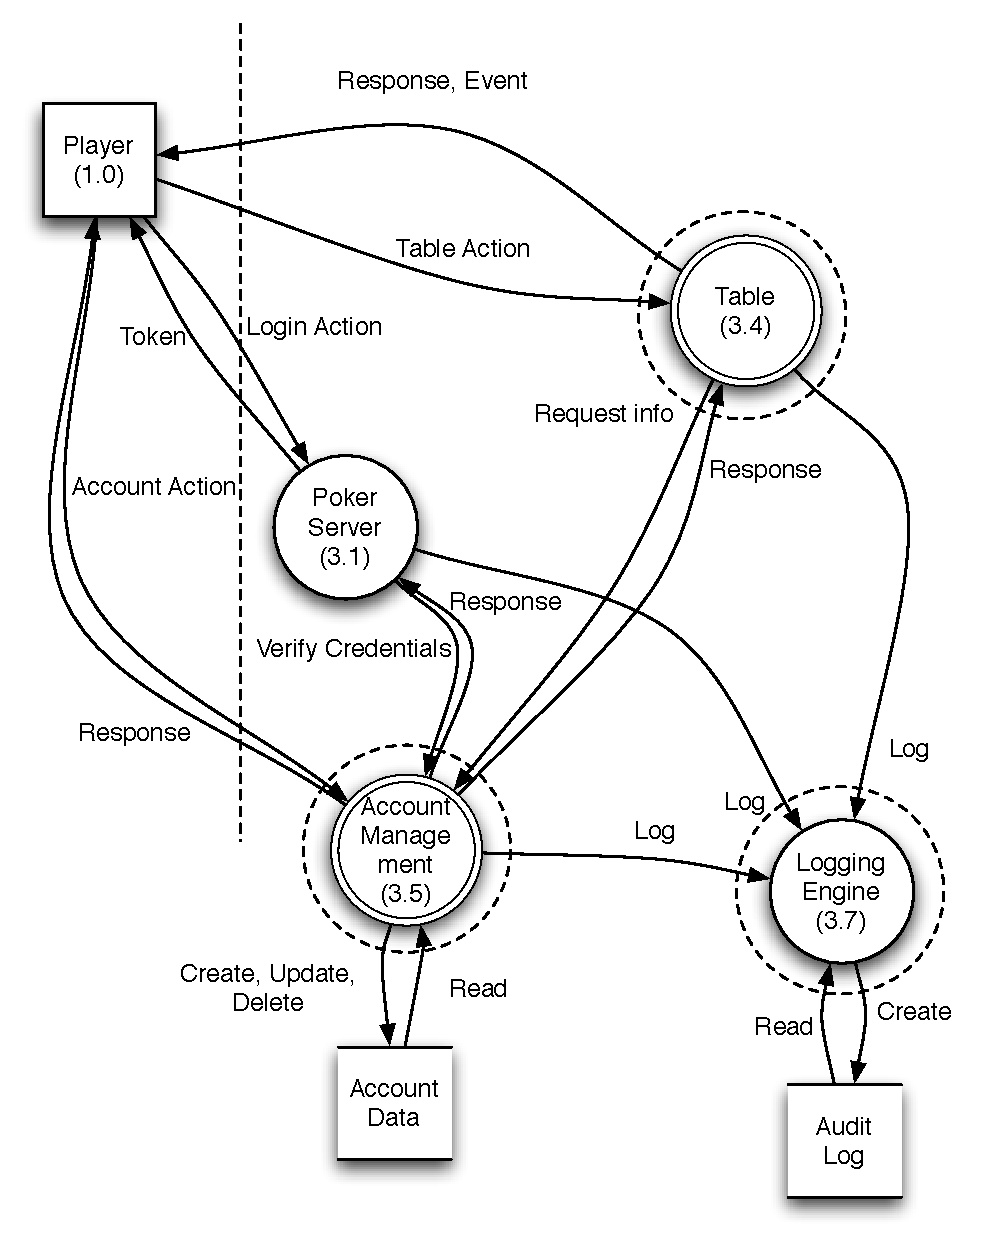
\includegraphics[scale=0.8]{dfd_level_0_player_simplified}
  \end{center}
  \caption{DFD Level-0 - only player - simplified}\label{fig:dfd_level_0_player_simplified}
\end{figure}
\begin{figure}[htpb]
  \begin{center}
    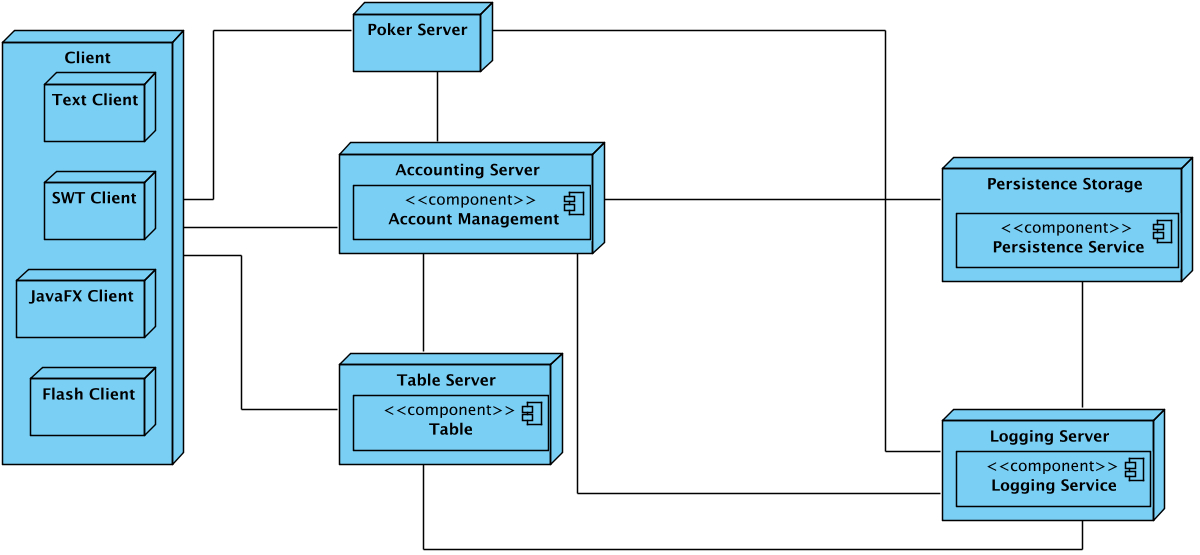
\includegraphics[angle=90,scale=0.65]{deployment_simplified.png}
  \end{center}
  \caption{Deployment View - simplified}\label{fig: deployment_simplified}
\end{figure}

\section{Security Objectives}
\label{MUCLabels}
In this section, we list all security objectives together with the misuse cases that are associated with them. The objectives are ordered by importance based on the number of associated misuse cases.

\subsection{Authentication (26 MUCs)}
\begin{enumerate}
\item Spoofing a player
\item Repudiation of a player
\item Spoofing the poker server
\item Tampering with the poker server
\item Repudiation of the poker server
\item Information disclosure at the poker server
\item Elevation of privilege at the poker server
\item Spoofing a table
\item Tampering with a table
\item Repudiation of a table
\item Information disclosure at a table
\item Elevation of Privilege at the table
\item Spoofing the account management system
\item Tampering with the account management system
\item Repudiation of using the account management system
\item Information disclosure of the account management system
\item Elevation of Privilege at the account management system
\item Spoofing the logging engine
\item Tampering with the logging engine
\item Repudiation of using the logging engine
\item Information disclosure of the logging engine
\item Elevation of Privilege at the logging engine
\item Tampering with the audit log
\item Information disclosure of the audit log
\item Tampering with account data
\item Information disclosure of account data
\end{enumerate}

\subsection{Authorization (21 MUCs)}
\begin{enumerate}
\item Repudiation of a player
\item Tampering with the poker server
\item Repudiation of the poker server
\item Information disclosure at the poker server
\item Elevation of privilege at the poker server
\item Tampering with a table
\item Repudiation of a table
\item Information disclosure at a table
\item Elevation of Privilege at the table
\item Tampering with the account management system
\item Repudiation of the account management system
\item Information disclosure of the account management system
\item Elevation of Privilege at the account management system
\item Tampering with the logging engine
\item Repudiation of the logging engine
\item Information disclosure of the logging engine
\item Elevation of Privilege at the logging engine
\item Tampering with the audit log
\item Information disclosure of the audit log
\item Tampering with account data
\item Information disclosure of account data
\end{enumerate}

\subsection{Application Integrity (12 MUCs)}
\label{ApplicationIntegrityMUCs}
\begin{enumerate}
\item Tampering with the poker server
\item Information disclosure at the poker server
\item Elevation of privilege at the poker server
\item Tampering with a table
\item Information disclosure at a table
\item Elevation of Privilege at the table
\item Tampering with the account management system
\item Information disclosure of the account management system
\item Elevation of Privilege at the account management system
\item Tampering with the logging engine
\item Information disclosure of the logging engine
\item Elevation of Privilege at the logging engine
\end{enumerate}

\subsection{Availability (10 MUCs)}
\begin{enumerate}
\item Denial of Service against the poker server
\item Denial of Service against a table
\item Denial of Service against the account management system
\item Denial of Service against the logging engine
\item Denial of Service against the audit log
\item Denial of Service against account data
\item Denial of Service of token requests
\item Denial of Service of tokens
\item Denial of Service of actions
\item Denial of Service of logging requests
\end{enumerate}

\subsection{Non-repudiation (6 MUCs)}
\begin{enumerate}
\item Repudiation of a player
\item Repudiation of the poker server
\item Repudiation of a table
\item Repudiation of the account management system
\item Repudiation of the logging engine
\item Repudiation of the audit log
\end{enumerate}

\subsection{Transmission Integrity (5 MUCs)}
\begin{enumerate}
\item Tampering with token requests
\item Tampering with tokens
\item Tampering with actions
\item Tampering with responses and events
\item Tampering with logging requests
\end{enumerate}

\subsection{Transmission Confidentiality (5 MUCs)}
\begin{enumerate}
\item Information Disclosure of token requests
\item Information Disclosure of tokens
\item Information Disclosure of actions
\item Information Disclosure of responses and events
\item Information Disclosure of logging requests
\end{enumerate}

\subsection{Auditing (4 MUCs)}
\begin{enumerate}
\item Repudiation of a player
\item Repudiation of the poker server
\item Repudiation of a table
\item Repudiation of the account management system
\end{enumerate}

\subsection{Storage Integrity (2 MUCs)}
\begin{enumerate}
\item Tampering with the audit log
\item Tampering with account data
\end{enumerate}

\subsection{Storage Confidentiality (2 MUCs)}
\begin{enumerate}
\item Information disclosure of the audit log
\item Information disclosure of account data
\end{enumerate}

\subsection{Application Confidentiality}
Application Confidentiality is not applicable since the code is open source.

\chapter{Securing the architecture}
\label{SecuringTheArchitecture}
\section{Quality trade-off labels}
\label{labels}
By analyzing the business goals, we constructed the following ordered list of quality trade-off labels (the ordering of this list is based on the relative importance of the different business goals):
\begin{description}
\item[Usability] The online casino has to be as easy to use as possible.
This quality attribute might seem less important than confidentiality and
integrity but in reality cheating will always happen (e.g. collusion) and
the loss will be calculated in. When a lot of people play in the online
casino because it is the most usable, this cost will be less significant.
\item[Confidentiality] It is important that certain information like the cards of a player, remains
confidential.
\item[Integrity] No one should be able to compromise the integrity of the application or it's data.
\item[Accountability] No player may be able to repudiate any bets or other actions.
\item[Manageability] The application must be easy to manage by an admin.
\item[Cost] The cost of the application should be reasonable to low, so profit will remain solid.
\item[Performance] Performance being the possible amount of games played simultaneously, is important because it
determines the maximum profit. It is very easy to come up with solutions
to performance problems because of the distributed nature of the
application (tables are independent).
\item[Maintainability] The application should be easy to maintain.
\end{description}
These labels will be used to guide the selection of security patterns in the next section: only the patterns that match best with these labels, will be selected.

\section{Pattern-based Methodology}
We will use the security patterns and methodology described in \cite{yskout} to select the appropriate patterns
for this application.

\subsection{Analysis Phase}
The analysis phase consists of eliciting the security requirements and annotating each
security requirement with the security object it belongs to. The security requirements have been elicited by the misuse cases
in secton \ref{MisUseCases}. The annotations to indicate for each misuse case to which security objective it belongs
are given in section \ref{MUCLabels}.


\subsection{Architecture Phase}
As stated in \cite[p13]{yskout}, the architecture of the system is designed using Attribute-Driven Design or ADD,
meaning it is created based on the non-functional requirements of the application and their relative importance.
Therefore a prioritized list of quality attributes, inspired by the business goals, was formulated under
section \ref{labels}. Then we iterate over the selection of architectural patterns, as it is stated by the methodology.

\subsubsection{Patterns already present}
\label{pres_patterns}
There are some security patterns that are already present in the architecture:
\begin{itemize}
\item Credential Tokenizer: The poker server is in a certain way a credential tokenizer: it provides a token to a
player, that the player can use to authenticate himself with the other processes.
\item Secure Service Facade: Every process has it's own facade where all the needed
security checks happen.
\item Secure Logger: the Logging Engine performs the tasks of a Secure Logger.
\end{itemize}

\subsubsection{Authentication}
\label{ArchitectureAuthentication}
The authentication requirement covers the most misuse cases so it is selected as the first requirement to cover.

The following patterns address authentication at the architectural level:
\begin{itemize}
\item Authentication Enforcer
\item Credential Tokenizer
\item Security Association
\item Secure Service Facade
\item Session
\item Single Access Point
\end{itemize}

Credential Tokenizer and Secure Service Facade are already present in the architecture.

Since these two patterns do not sufficiently cover Authentication, we continue with the set of patterns that aren't
present yet: Authentication Enforcer, Security Association, Session and Single Access Point.

There are no patterns in this list that conflict with any existing patterns.
Next, we screen the short descriptions of the selected patterns to see if they are applicable.
\begin{itemize}
\item Security Association appears to be missing from the list and is therefore discarded.
\item Session won't be selected, because there is too little shared state between the different processes. State is almost only shared within a process. One could consider the use of tokens to maintain an autenticaton state as an instantiation of Session. Because the state in that case is very limited we choose not to.
\end{itemize}

The other patterns seem applicable:
\begin{itemize}
\item Authentication Enforcer has as labels +Maintainability, +Manageability, +Auditability, -Anonymity, +Privacy,
+Accountability, +Portability, benefits from Secure Pipe and Secure Service Facade and has as alternative
Container Managed Security.
\item Single Access Point has as labels +Manageability and has no relations with other patterns.
\end{itemize}

Clearly Authentication Enforcer is the better choice here: its labels match better with the quality trade-off labels
than Single Access Point and it benefits from the Secure Service Facade pattern that already exist in the architecture.
Single Access Point would also lead to a too centralised architecture. Container Managed Security is a system pattern and will later be considered as an alternative for Authentication Enforcer.

The Authentication Enforcer pattern is selected to deal with the Authentication requirement. It is instantiated with a beneficial relationship from the existing security facades. It collaborates with Account Management to perform authentication.

We can now mark the Authentication requirement as resolved at the architectural level.

\subsubsection{Authorization}

The following patterns address authorization at the architectural level:
\begin{itemize}
\item Authorization Enforcer
\item Controlled Object Monitor
\item Full View With Errors
\item Limited View
\item Secure Service Facade
\item Single Access Point
\end{itemize}

Secure Service Facade is already present in the architecture.
Single Access Point was already considered under Authentication and was not selected.

The candidates for selection are Authorization Enforcer, Controlled Object Monitor, Full View With Errors
and Limited View.

There are no patterns in this list that conflict with any existing patterns.
Next, we screen the short descriptions of the selected patterns to see if they are applicable.
\begin{itemize}
\item Controlled Object Monitor isn't applicable because there are few shared objects between processes so
there is little need to monitor and intercept access requests from different processes to objects.
\end{itemize}
The other patterns seem applicable:
\begin{itemize}
\item Authorization Enforcer has as labels +Maintainability, +Manageability, +Auditability, +Accountability and
+Portability, benefits from Authentication Enforcer and Secure Service Facade and has as alternative
Container Managed Security.

\item Full View With Errors has as labels +Maintainability, -Usability and conflicts with Limited View and has as
alternative Limited View.

\item Limited View has as labels +Usability and conflicts with Full View With Errors and has as alternative Full View
With Errors.
\end{itemize}

Authorization Enforcer will be selected, because it has many + labels that match the quality trade-off labels and
it benefits from already instantiated patterns such as Authentication Enforcer and Secure Service Facade. Its
alternative, Container Managed Security, is a system pattern and will be consider later. Maybe we will have to
backtrack over the choices we made if the alternative appears to be a better choice.

Both Limited View and Full View with Errors will be selected, but for different parts so there is no conflict.
Limited View will be used for the client side, because Usability for the clients is a major issue. Full View with
Errors will be used for the server API because it is technically the only possibility at this level.

The Authorization Enforcer, Limited View and Full View With Errors are selected to deal with the Authorization requirement. The Authorization Enforcer is instantiated with a beneficial relationship from the existing Secure Service Facade. It uses the Authentication Enforcer to authenticate a user. Limited View will be enforced on each client by some certification process or coding guidelines (as anyone can write a client for our server). The server itself will only be able to instantiate the Full View With Errors as it's the only possibility.

We can now consider the Authorization requirement as resolved at the architectural level.

\subsubsection{Application Integrity}
\label{ArchitecturalApplicationIntegrity}
The following patterns address application integrity at the architectural level:
\begin{itemize}
\item Checkpointed System
\item Comparator-Checked Fault-Tolerant System
\end{itemize}

There are no patterns in this list that conflict with any existing patterns.
Next, we screen the short descriptions of the selected patterns to see if they are applicable. Both patterns seem
applicable.

\begin{itemize}
\item Checkpointed System has as labels +Dependability, -Performance and -Cost , and benefits from Comparator Checked
 Fault Tolerant System and impairs Audit Interceptor.

\item Comparator-Checked Fault-Tolerant System has as labels -Cost, -Performance, +Dependability and impairs Audit
Interceptor and has as alternative Output Guard and benefits from Checkpointed System.
\end{itemize}

Checkpointed System would be useful to implement in the Cashier process, even though it has a negative influence on both the Cost and the Performance,
because there must be a way to recover from a crash of a critical process such as Cashier. The Cashier process
will be checkpointed: the cashier will reserve the money used in bets of a deal. When the deal ends, the table
will tell the cashier the money can be really transfered. If for some reason, the table fails and the deal is
cancelled, the money used in that deal will go back to its owners.


Comparator-Checked Fault-Tolerant System won't be selected because it is considered overkill (very high cost) and has too few
advantages compared to its disadvantages.

Due to a lack of patterns to tackle the problem, we must leave Application Integrity as it is.

\subsubsection{Accountability}

The following patterns address accountability at the architectural level:

\begin{itemize}
\item Secure Logger
\end{itemize}
Secure Logger is already present in the architecture. The Accountability requirement is considered as solved at the architectural level.

\subsubsection{Data Integrity}
The following patterns address data integrity at the architectural level:
\begin{itemize}
\item Session
\item Secure Access Layer
\item Secure Pipe
\end{itemize}

There are no patterns in this list that conflict with any existing patterns.
Next, we screen the short descriptions of the selected patterns to see if they are applicable.
\begin{itemize}
\item Session was already dropped in section \ref{ArchitectureAuthentication} because there is very little
shared state.
\end{itemize}
The other patterns seem applicable:
\begin{itemize}
\item Secure Access Layer has as labels +Maintainability and +Portability, and has no relations with other patterns.

\item Secure Pipe has no labels in the list, but we believe it should have +Confidentiality and +Integrity. The pattern
benefits from Secure Association (which by the way is not included in the list, see \ref{Criticism}).
\end{itemize}

Secure Access Layer will be selected because it has only positive labels and has no relation with other patterns.
Secure Pipe will also be selected because confidentiality and integrity are considered important quality labels.

Secure Access Layer and Secure Pipe are selected to deal with the Data Integrity requirement. Secure Access Layer is instantiated before the persistence service to cope with future changes and to provide a uniform interface. Secure Pipes are instantiated wherever communication occurs over the wire (e.g. with SSL).

We can now consider the Data Integrity requirement as resolved at the architectural level.
\subsubsection{Availability}
The following patterns address availability at the architectural level:
\begin{itemize}
\item Checkpointed System
\item Load Balancer
\item Replicated System
\end{itemize}

Checkpointed System has already been selected for use in the Cashier when Application Integrity was considered.

There are no patterns in this list that conflict with any existing patterns.
Next, we screen the short descriptions of the selected patterns to see if they are applicable. Both patterns seem
applicable.

\begin{itemize}
\item Load Balancer has as label +Performance and benefits from Replicated System and Session Failover. It impairs
Session.
\item Replicated System has as labels -Manageability and -Cost and depends on Load Balancer.
\end{itemize}

Load Balancer is selected, because it has a positive influence on the performance. The nature of the application
makes it also easy to distribute the load. Different tables can for instance be located at different servers and the lobby can be used as a central registry.

Replicated System isn't selected, because the cost of replicating all the components would be too great compared
to the benefits.

Load Balancer is selected to deal with the Availability requirement. It is instantiated in the poker server and should collaborate with the lobby component, that is omitted for this analysis, to balance the load between all table servers. The table server can easily be spread over multiple servers because most game tables are independent.

We can now consider the Availability requirement as resolved at the architectural level.

\subsection{Design Phase}
We don't consider design phase patterns because it isn't part of the assignment and it would be too
low level.

\subsection{System Phase}

\subsubsection{Authentication}
The following patterns handle Authentication at the system level:
\begin{itemize}
\item Container Managed Security
\end{itemize}

As mentioned before, Container Managed Security is an alternative to Authentication and Authorization Enforcer.
If we decided to select and instantiate Container Managed Security we could backtrack over the choices we made
after the selection of Authentication and Authorization Enforcer.

\begin{itemize}
\item Container Managed Security has as labels +Manageability, +Portability, +Integrity and is an alternative for
Authentication and Authorization Enforcer.
\end{itemize}

Container Managed Security won't be selected because we don't have a J2EE or any other container and Authentication
and Authorization Enforcer offer more benefits and flexibility.

\subsubsection{Authorization}
The following patters handle Authorization at the system level:
\begin{itemize}
\item Application Firewall
\item Container Managed Security
\item Controlled Process Creator
\item Controlled Object Factory
\item Demilitarized Zone
\item Firewall
\end{itemize}

There is no pattern that conflicts with earlier instantiated patterns.
Some patterns aren't applicable:
\begin{itemize}
\item Controlled Process Creator isn't really applicable because there are no processes that are created at runtime.
At a lower level there are ofcourse thread pools and database connection pools that control the creation of those
processes. We will not consider them as instantiations of the Controlled Process Creator pattern here but it
might be up for discussion.
\item Controlled Object Factory depends on Controlled Object Monitor, which was discarded earlier.
\end{itemize}
The other patterns seem applicable:
\begin{itemize}
\item Application Firewall has as labels -Performance, +Manageability, +Auditability and has as alternative Input Guard.
\item Demilitarized Zone has as labels -Performance, -Cost, -Manageability, -Dependability, +Maintainability and depends
on Firewall.
\item Firewall has as labels +Accountability, -Performance, -Dependability and benefits from Demilitarized Zone and
Application Firewall.
\end{itemize}

Application Firewall is selected and instantiated because auditability is an important quality label compared to
the performance penalty.
Demilitarized Zone isn't selected because of the high cost and because a demilitarized zone doesn't seem useful if the only task of the front end is to forward request. The processes that are placed outside of the secure zone should at least be performing some kind of non-trivial computation for them to pose enough of a risk to require a DMZ.
Firewall is selected and because Accountability is an important quality label, and the pattern benefits
from the previously instantiated Application Firewall.

So Application Firewall and Firewall are selected to deal with Authorization at the system level. Application Firewall is instantiated at the poker server to log all incoming request for auditing and filter out all invalid input. The firewall is instantiated before the poker server to counter flooding and to be able to ban IPs.

We now consider Authorization at the system level covered.
\subsubsection{Application Integrity}
There are no patterns that deal with application integrity at the system level.

\subsubsection{Accountability}
The following patterns handle Accountability at the system level:
\begin{itemize}
\item Audit Interceptor
\end{itemize}

Audit Interceptor doesn't conflict with any earlier instantiated pattern and seems applicable.

\begin{itemize}
\item Audit Interceptor has as labels -Performance, +Auditability, +Maintainability, +Manageability and depends on
Secure Logger and benefits from Secure Service Facade.
\end{itemize}

Audit Interceptor is selected and instantiated because Auditability and Maintainability are important quality
labels and it benefits from the Secure Service Facade, which was already present. The depends relation with
Secure Logger is already dealt with because the latter pattern was already present.

We now consider Accountability at the system level as covered.

\subsubsection{Data Integrity}
The following patterns handle Data Integrity at the system level:
\begin{itemize}
\item Secure Message Router
\end{itemize}

Secure Message Router doesn't conflict with any previously instantiated pattern and seems applicable:

\begin{itemize}
\item Secure Message Router has as labels +Manageability, +Maintainability, +Confidentiality, +Integrity, -Availability
and has no relations with other patterns.
\end{itemize}

Secure Message Router might be useful if there would be the need to interact safely with an external payment system
but we don't consider it here, in our simplified version.
\subsubsection{Availability}
There are no patterns who handle availability at the system level.
\subsection{Instantiated Patterns}
\label{inst_patterns}
To summarize, here is the list of the instantiated patterns, that weren't present yet in the architecture:
\begin{itemize}
\item Authentication Enforcer
\item Authorization Enforcer
\item Secure Pipe
\item Full View with Errors
\item Limited View
\item Application Firewall
\item Firewall
\item Checkpointed System
\item Audit Interceptor
\item Secure Access Layer
\item Load Balancer
\end{itemize}

\section{Final security enhanced architecture}
By following the steps in the pattern-based approach described in the previous section the vanilla architecture has been enhanced with security related components. The decomposition view can be found in figure \ref{fig:decomposition_secured}. The deployment view in figure \ref{fig:deployment_secured}.

\begin{figure}[htpb]
  \begin{center}
    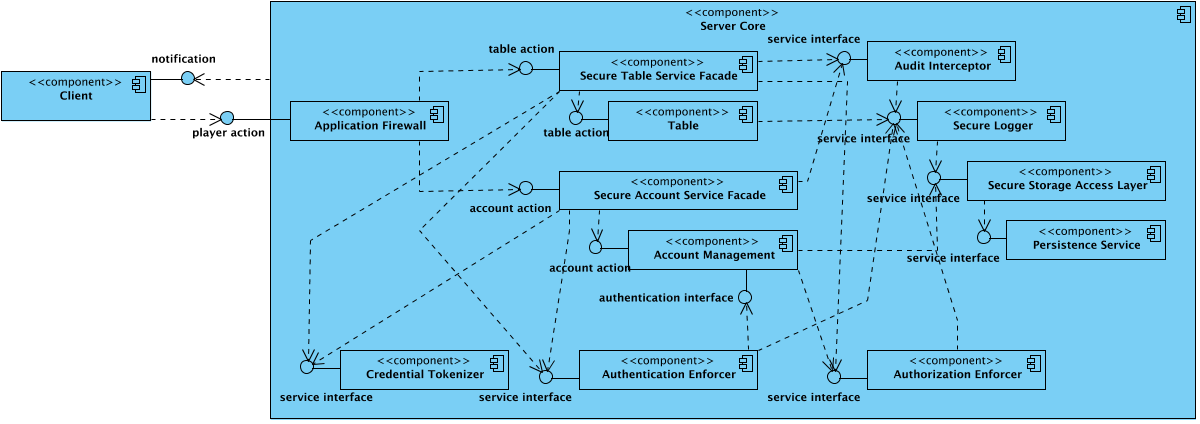
\includegraphics[angle=90,scale=0.65]{component_secured.png}
  \end{center}
  \caption{Decomposition View - Security Enhanced Architecture}\label{fig:decomposition_secured}
\end{figure}

\begin{figure}[htpb]
  \begin{center}
    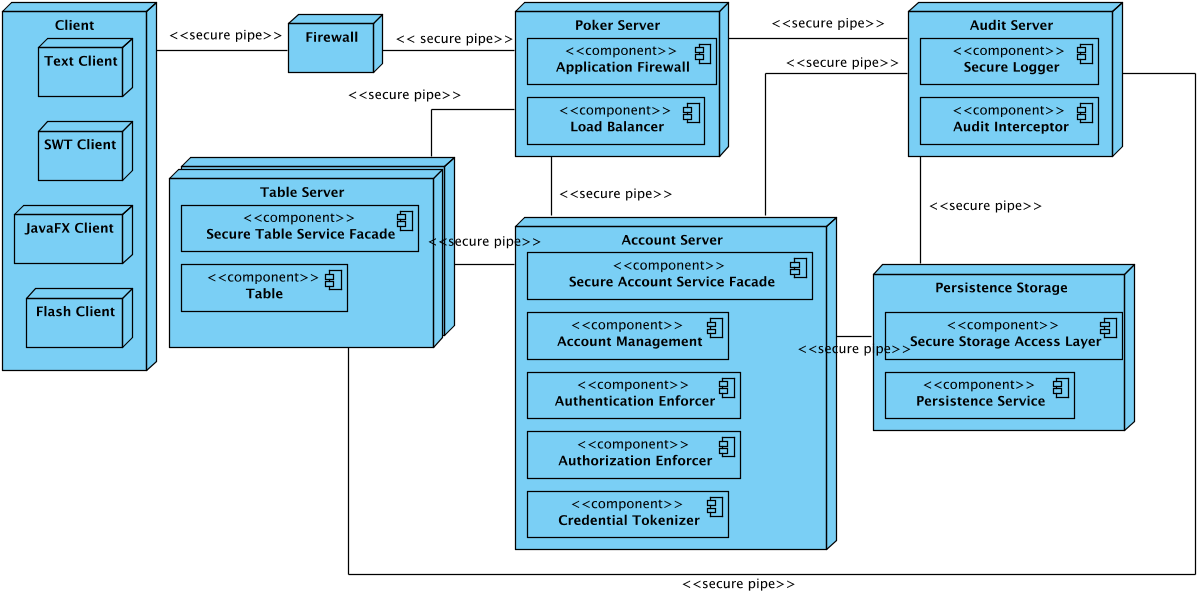
\includegraphics[angle=90,scale=0.65]{deployment_secured.png}
  \end{center}
  \caption{Deployment View - Security Enhanced Architecture}\label{fig:deployment_secured}
\end{figure}

\section{GAP Analysis: Coverage of Security Patterns vs Misuse Cases}
In this section we will evaluate the security enhanced architecture to verify how good this new architecture mitigates all threats identified in chapter \ref{IdentifyingThreats}. In tables \ref{table:gap1} and \ref{table:gap2} the coverage of every misuse case is elicited by documenting the security patterns that mitigate the corresponding threat.
\begin{table}[htpb]
\begin{center}
\begin{tabular}{| p{5cm} | p{10,5cm} |}
\hline
\textbf{Misuse Case} 	& \textbf{Coverage} \\
\hline
\hline
\textbf{Player} & \\\hline
Spoofing a player & Authentication enforcer, Credential tokenizer \\\hline
Repudiation of a Player & Secure logger, Audit interceptor, Secure service facade, Secure Pipe \\\hline
\textbf{Poker Server} & \\\hline
Spoofing the poker server & Authentication enforcer, Authorization enforcer, Secure service facade \\\hline
Tampering with the poker server & Authentication enforcer, Authorization enforcer, Secure service facade, Credential tokenizer, Secure pipe, Application firewall \\\hline
Repudiation of the poker server & Secure logger, Audit interceptor, Secure pipe, Secure service facade\\\hline
Information disclosure at the poker server & Secure Pipe, Authentication Enforcer, Authorization Enforcer, Secure Service Facade, Credential tokenizer, Application firewall \\\hline
DoS against the poker server & Application Firewall, Firewall, Audit interceptor, Secure logger\\\hline
Elevation of privilege at the poker server & Authentication Enforcer, Authorization Enforcer, Secure Service Facade, Credential Tokenizer, Secure pipe, Application firewall \\\hline
\textbf{Table} & \\\hline
Spoofing a table & Authentication enforcer, Authorization enforcer, Secure service facade \\\hline
Tampering with a table & Authentication enforcer, Authorization enforcer, Secure service facade, Credential tokenizer, Secure pipe, Application firewall \\\hline
Repudiation of an action at a table & Secure logger, Audit interceptor, Secure pipe, Secure service facade\\\hline
Information disclosure at a table & Secure Pipe, Authentication Enforcer, Authorization Enforcer, Secure Service Facade, Credential tokenizer, Application firewall \\\hline
DoS against a table & Load balancer, Application Firewall, Firewall, Audit interceptor, Secure logger\\\hline
Elevation of privilege at a table & Authentication Enforcer, Authorization Enforcer, Secure Service Facade, Credential Tokenizer, Secure pipe, Application firewall \\\hline
\end{tabular}
\end{center}
\caption{GAP Analysis - 1}
\label{table:gap1}
\end{table}

\begin{table}[htpb]
\begin{center}
\begin{tabular}{| p{5cm} | p{10,5cm} |}
\hline
\textbf{Misuse Case} 	& \textbf{Coverage} \\
\hline
\hline
\textbf{Account Management} & \\\hline
Spoofing the account management system & Authentication enforcer, Authorization enforcer, Secure service facade \\\hline
Tampering with the account management system & Authentication enforcer, Authorization enforcer, Secure service facade, Credential tokenizer, Secure pipe, Application firewall \\\hline
Repudiation of using the account management system & Secure logger, Audit interceptor, Secure pipe, Secure service facade\\\hline
Information disclosure of the account management system & Secure Pipe, Authentication Enforcer, Authorization Enforcer, Secure Service Facade, Credential tokenizer, Application firewall \\\hline
DoS against the account management system & Application Firewall, Firewall, Audit interceptor, Secure logger\\\hline
Elevation of privilege at the account management system & Authentication Enforcer, Authorization Enforcer, Secure Service Facade, Credential Tokenizer, Secure pipe, Application firewall \\\hline
\textbf{Logging Engine} & \\\hline
Spoofing the logging engine & Authentication enforcer, Authorization enforcer, Secure service facade \\\hline
Tampering with the logging engine & Authentication enforcer, Authorization enforcer, Secure service facade, Credential tokenizer, Secure pipe, Application firewall \\\hline
Repudiation of using the logging engine & Secure pipe, Secure service facade \\\hline
Information disclosure at the logging engine & Authentication Enforcer, Authorization Enforcer, Secure Service Facade, Credential Tokenizer, Secure pipe, Application firewall \\\hline
\textbf{Audit Log} & \\\hline
Tampering with the audit log & Authentication enforcer, Authorization enforcer, Secure service facade, Credential tokenizer, Secure pipe, Application firewall \\\hline
Repudiation of logging something in the audit log & Secure pipe, Secure service facade \\\hline
Information disclosure of the audit log & Secure Pipe, Authentication Enforcer, Authorization Enforcer, Secure Service Facade, Credential tokenizer, Application firewall \\\hline
DoS against the audit log & Application Firewall, Firewall \\\hline
\textbf{Account Data} & \\\hline
Tampering with account data & Authentication enforcer, Authorization enforcer, Secure service facade, Credential tokenizer, Secure pipe, Application firewall \\\hline
Information disclosure of account data & Secure Pipe, Authentication Enforcer, Authorization Enforcer, Secure Service Facade, Credential tokenizer, Application firewall \\\hline
DoS against account data & Application Firewall, Firewall, Audit interceptor, Secure logger\\\hline
\end{tabular}
\end{center}
\caption{GAP Analysis - 2}
\label{table:gap2}
\end{table}

\begin{table}[htpb]
\begin{center}
\begin{tabular}{| p{5cm} | p{10,5cm} |}
\hline
\textbf{Misuse Case} 	& \textbf{Coverage} \\
\hline
\hline
\textbf{Business Misuse Cases} & \\\hline
A malicious player uses multiple accounts to access more hidden cards & Partially covered: authentication enforcer, credential tokenizer \\\hline
A malicious player with admin rights misuses his privileges & Partially covered: authorization enforcer. Add a policy that makes it impossible to access card data from ongoing game. \\\hline
A malicious player misuses the right to ask the admin to view the log of the table & Currently not covered (not part of the architecture) \\\hline
A malicious player can flood the network of another player to force a time-out & Currently not covered (not part of the architecture), but time-out policy should try to minimize possible misuse. \\\hline
Collusion & Partially covered: Secure logger, Audit interceptor, Secure service facade, Secure Pipe \\\hline
An admin collaborates with a player to play with full information disclosure & Partially covered: authorization enforcer. Add a policy that makes it impossible to access card data from ongoing game. \\\hline
Malicious player can predict hole and community cards & Currently not covered (not part of the architecture) \\\hline
Chip dumping & Partially covered: Secure logger, Audit interceptor, Secure service facade, Secure Pipe \\\hline
Placing spyware on the computer systems of honest players & Currently not covered (not part of the architecture) \\\hline
Altered client provided to the players & Currently not covered (not part of the architecture) \\\hline
\end{tabular}
\end{center}
\caption{GAP Analysis - 3}
\label{table:gap3}
\end{table}

\chapter{Evaluating the architecture}
\label{Evaluation}

\section{Identified Architectural Approaches}
\subsection{Architectural Patterns}
Based on \cite{Avgeriou2005}, we identified the following patterns in the architecture:
\begin{itemize}
\item \textbf{Layers:} A layered structure can be identified for exception handling and communication.
\item \textbf{Broker:} The main server can be seen as a broker for the different backend components: lobby, table and account management.
\item \textbf{Microkernel:} The table is a microkernel to provide different game types e.g. Omaha and Texas Hold'em.
\item \textbf{Model-View-Controller:} At the client side, we have a variation on MVC: the model part is located
at the server, the controller consists of the event listeners who adapt the view based on the incoming events and
the views display the information on the screen.
\item \textbf{Client-Server:} The server handles requests from multiple clients.
\item \textbf{Remote Procedure Calls:} Remote Procedure calls are used for the interaction between client and server.
\item \textbf{Publish-Subscribe:} Interested clients can register themselves to receive specific events from the server.
\item \textbf{Message Queuing:} When an event can not be sent immediately, the event is queued until the receiver can accept it.
\end{itemize}

\subsection{Security Patterns}
The security patterns are just the sum of the ones that were already present in the architecture
(\ref{pres_patterns}) and the ones that were instantiated in \ref{inst_patterns}:
\begin{itemize}
\item Authentication Enforcer
\item Authorization Enforcer
\item Secure Pipe
\item Full View with Errors
\item Limited View
\item Application Firewall
\item Firewall
\item Checkpointed System
\item Audit Interceptor
\item Secure Access Layer
\item Load Balancer
\item Credential Tokenizer
\item Secure Service Facade
\item Secure Logger
\end{itemize}
For a more in depth description of these patterns see chapter \ref{SecuringTheArchitecture}.

\section{Quality Attribute Tree}
From the business goals identified in the initial architecture, the following important quality attributes are 
selected:  \textbf{usability}, \textbf{security} and \textbf{availability}. These three were selected because
they represent the most important business goals. The overview of the quality attribute 
tree can be found in table \ref{QAT}. In the following sections the rationale for choosing the importance 
(business perspective) and difficulty (technical perspective) ratings are elaborated.
\begin{table}[htpb]
\begin{center}
\begin{tabular}{| p{2,2cm} | p{0.25cm}  p{2.5cm} | p{0.55cm}  p{7cm} | p{0,31cm} | p{0,31cm} | }
\hline
\textbf{Level 2:\newline Quality\newline Attribute} & \multicolumn{2}{p{2.75cm}|}{\textbf{Level 3:\newline Quality\newline Attribute\newline Refinement}} & \multicolumn{2}{p{6.65cm}|}{\textbf{Level 4:\newline Quality Attribute Scenario}} & \textbf{I} & \textbf{D}\\
\hline
\hline
\textbf{Availability} 	& A1 & Prevention 	& A1.1 & The MTBF of all hard disks is at least 1 month. & H & M   \\\cline{4-7}
			& &			& A1.2 & Network connections have a MTBF of 3 months.  & H & M  \\\cline{2-7}
			& A2 & Fault\newline detection 	& A2.1 & Server hard disk failure is detected within 20s. & M & M  \\\cline{4-7}
			& &			& A2.2 & Network failure is detected within 5s. & M & M  \\\cline{2-7}
			& A3 & Recovery 	& A3.1 & Recovery from server hard disk failure takes 50s and succeeds 99.99\% of the time. & M & H  \\\cline{4-7}
			& &			& A3.2 & Recovery from a network failure takes 30s and succeeds 99.99\% of the time. & M & H  \\\hline
\textbf{Security} 	& S1 & Authentication 	& S1.1 & 99.999\% of all users are correctly authenticated. & H & M   \\\cline{2-7}
			& S2 & Authorization 	& S2.1 & 99.999\% of all user actions are correctly authorized. & H & M  \\\cline{2-7}
			& S3 & Storage\newline Confidentiality & S3.1 & All account related data are secure 99.999\% of time. & H & L   \\\cline{2-7}
			& S4 & Transmission\newline Confidentiality & S4.1 & Cards are transmitted secure 99.999\% of time. & M & L  \\\cline{2-7}
			& S5 & Transmission\newline Integrity & S5.1 & 99.999\% of all transmitted cards remain unmodified. & M & L  \\\cline{4-7}
			& &			& S5.2 & 99.999\% of all transmitted actions remain unmodified. & H & L  \\\cline{2-7}
			& S6 & Auditing 		& S6.1 & 99.999\% of actions are logged and kept for 2 years. & L & M  \\\hline
\textbf{Usability} 	& U1 & Learnability & U1.1  & The user must be able to be seated and play at a table within 3 mouse clicks the first time they use the application. & L & L  \\\cline{2-7}
			&U2 &Efficiency			&U2.1  &At each screen, the user must be able to find the correct button for his action, within 2 seconds. & H & L  \\\cline{2-7}
			&U3 &Satisfaction			&U3.1  &The user must be able to define default actions for certain situations (e.g. default check/fold as action in the current game).& M & L  \\\cline{4-7}
			& &			&U3.2  &The user interface must respond to an action of the user within 2 seconds. & H & M  \\\cline{2-7}
			&U4 &Adaptability			&U4.1  &The user interface must be separated from the rest of the application to enable fast and easy usability testing. & M & M  \\\hline

\end{tabular}
\end{center}
\caption{Quality Attribute Tree}
\label{QAT}
\end{table}

\subsection{Availability}
\begin{itemize}
\item[\textbf{A1.1}] The MTBF\footnote{Mean Time Between Failures} of all hard disks is at least 1 month.
\begin{itemize}
\item Importance: High. It's more important to prevent failure than recovering from failure.
\item Difficulty: Medium. Very reliable hardware is available.
\end{itemize}
\item[\textbf{A1.2}] Network connections have a MTBF of 3 months.
\begin{itemize}
\item Importance: High. It's more important to prevent failure than recovering from failure.
\item Difficulty: Medium. Very reliable networking hardware is available.
\end{itemize}
\item[\textbf{A2.1}] Server hard disk failure is detected within 20s.
\begin{itemize}
\item Importance: Medium. It's important, but less important than preventing failures.
\item Difficulty: Medium. There is software available for the detection of hard disk failures.
\end{itemize}
\item[\textbf{A2.2}] Network failure is detected within 5s.
\begin{itemize}
\item Importance: Medium. It's important, but less important than preventing failures.
\item Difficulty: Medium. There are several architectural patterns that cover this issue.
\end{itemize}
\item[\textbf{A3.1}] Recovery from server hard disk failure takes 50s and succeeds 99.99\% of the time.
\begin{itemize}
\item Importance: Medium. Recovery should have the same importance as detection.
\item Difficulty: High. Some hardware components are difficult to replace.
\end{itemize}
\item[\textbf{A3.2}] Recovery from a network failure takes 30s and succeeds 99.99\% of the time.
\begin{itemize}
\item Importance: Medium. Recovery should have the same importance as detection.
\item Difficulty: High. It's difficult to recover from failure in a distributed system as there are synchronization issues.
\end{itemize}
\end{itemize}

\subsection{Security}
\begin{itemize}
\item[\textbf{S1.1}] 99.999\% of all users are correctly authenticated.
\begin{itemize}
\item Importance: High. It's important all users are correctly identified.
\item Difficulty: Medium. There are several reusable components and patterns available for authentication.
\end{itemize}
\item[\textbf{S2.1}] 99.999\% of all user actions are correctly authorized.
\begin{itemize}
\item Importance: High. It's important users can only do what they are allowed to do.
\item Difficulty: Medium. There are several reusable components and patterns available for authorization.
\end{itemize}
\item[\textbf{S3.1}] All account related data are secure 99.999\% of time.
\begin{itemize}
\item Importance: High. It's important all sensitive user data are only accessible for authorized persons.
\item Difficulty: Low. This relies on the correct authorization discussed in S2.1 and on secure storage.
\end{itemize}
\item[\textbf{S4.1}] Cards are transmitted secure 99.999\% of time.
\begin{itemize}
\item Importance: Medium. It's important all card info are transmitted secure, but it's less important than correct authorization. 
\item Difficulty: Low. This can easily be achieved through the use of a secure pipe.
\end{itemize}
\item[\textbf{S5.1}] 99.999\% of all transmitted cards remain unmodified.
\begin{itemize}
\item Importance: Medium. It's important all card info are transmitted unmodified, but it's less important than correct authorization. 
\item Difficulty: Low. This can easily be achieved through the use of a secure pipe.
\end{itemize}
\item[\textbf{S5.2}] 99.999\% of all transmitted actions remain unmodified.
\begin{itemize}
\item Importance: High. It's important all actions are transmitted unmodified, as it can lead to incorrect authorization.
\item Difficulty: Low. This can easily be achieved through the use of a secure pipe.
\end{itemize}
\item[\textbf{S6.1}] 99.999\% of actions are logged and kept for 2 years.
\begin{itemize}
\item Importance: Low. This is a legal constraint and should be available, but it's not critical for providing a good service to the player. 
\item Difficulty: Medium. This can be implemented with the use of security patterns, but there may be a problem with a feature interaction between logging and confidentiality.
\end{itemize}
\end{itemize}

\subsection{Usability}
\begin{itemize}
\item The user must be able to be seated and play at a table within 3 mouse clicks the first time they use
the application.
\begin{itemize}
\item Importance: High. It is critical that new players easily find their way to the poker tables, or else
they might prefer other poker applications.
\item Difficulty: Low. A well designed user interface should accomplish this. This scenario can be easily tested by a number of usability tests (such as Think Aloud Protocol etc.).
\end{itemize}
\item At each screen, the user must be able to find the correct button for his action, within 2 seconds.
\begin{itemize}
\item Importance: Medium. If users have a hard time finding the right buttons, they might get annoyed and 
switch to other poker applications.
\item Difficulty: Low. Again a well designed user interface should take care of this, the user response time can be measured by a number of usability tests (such as Think Aloud Protocol etc.).
\end{itemize}
\item The user must be able to define default actions for certain situations (e.g. default check/fold as action
in the current game).
\begin{itemize}
\item Importance: Low. Some user that frequently perform the same actions, might want to automate those actions;
but those people are a smaller group and thus this is less important.
\item Difficulty: Low. This can be established using check-boxes etc.
\end{itemize}
\item The user interface must respond to an action of the user within 2 seconds.
\begin{itemize}
\item Importance: High. This quality attribute is very important, because a non-responsive user interface
will annoy many users, who might use other poker applications as a reaction.
\item Difficulty: Medium. This can be tackled by using a separate listener thread that dispatches the events
to other threads that handle them; however there can be some pitfalls here (e.g. when the user is playing 
a lot of different tables at the same time or when network problems occur)
\end{itemize}
\item The user interface must be separated from the rest of the application to enable fast and easy 
usability testing.
\begin{itemize}
\item Importance: Medium. Easier usability tests are very usefull to track the effect of small changes to
the user interface. This iteration will lead to a better user interface.
\item Difficulty: Medium. The seperation of user interface and system can be handled by some patterns like
Model-View-Controller; it requires some discipline, insight and experience from the developers to fully
accomplish this.
\end{itemize}
\end{itemize}

\section{Analysis of the architectural approaches}

\subsection{Availability}

\begin{tabular}{| p{4,5cm} | p{2,25cm} | p{2,25cm} | p{2,25cm} | p{2,25cm} | }
\hline
\textbf{Scenario \#:} & \multicolumn{4}{| p{9cm} |}{\textbf{The MTBF of all hard disks is at least 1 month.} } \\\hline
\textbf{Attribute(s)} & \multicolumn{4}{| p{9cm} |}{Availability} \\\hline
\textbf{Environment} & \multicolumn{4}{| p{9cm} |}{Normal Operations} \\\hline
\textbf{Stimulus} & \multicolumn{4}{| p{9cm} |}{A hard disk fails.} \\\hline
\textbf{Response} & \multicolumn{4}{| p{9cm} |}{Failure only occurs once every month.} \\\hline \hline
\textbf{Architectural Decision} & \textbf{Sensitivity} & \textbf{Tradeoff} & \textbf{Risk} & \textbf{Nonrisk}\\\hline
Broker  &  &  & R1 &   \\\hline 
Checkpointed System  & S2 & T2 & R2 &   \\\hline 
No Comparator-checked Fault-tolerant System   & S3 & T3 &  & NR3  \\\hline 
Load Balancer  & S4 & T4  & R4 &   \\\hline 
No Replicated System  & S5 & T5 &  & NR5  \\\hline 
Secure Logger  & S6 & T6 & R6 &   \\\hline 
Application Firewall  & S7 &  & R7 &   \\\hline 
\hline
\textbf{Architecture diagram} & \multicolumn{4}{| p{9cm} |}{See figures \ref{fig:decomposition_secured} and \ref{fig:deployment_secured}} \\\hline
\end{tabular}
\begin{itemize}
\item \textbf{R1:} Adding the level of indirection of a broker requires extra hardware. This adds a new point of failure to the entire system.
\item \textbf{S2, T2 \& R2:} Having a checkpointed system in the cashier server requires a lot of extra hardware utilization. The more fine grained the checkpoints, the more utilization and the larger the risk. There's a tradeoff with Dependability. 
\item \textbf{S3, T3, \& NR3:} By not choosing a comparator-checked fault-tolerant system, we do not incur the cost of adding the extra hardware that might also cause failure to occur. If we were to choose it, the number of replicated systems would increase the risk of hard disk failure. There's a tradeoff with Dependability.
\item \textbf{S4, T4 \& R4:} Every server in the load balancing setup of the table servers imposes an extra risk of hard disk failure. There's a tradeoff with the performance advantage the load balancer has.
\item \textbf{S5, T5 \& NR5:} Not replicating all the processes in the system reduces the probability that a hard disk will fail somewhere. There's a tradeoff with other aspects of Availability.
\item \textbf{S6, T6 \& R6:} The secure logger pattern brings with it the need for an extra data source, typically using hard drives for persistent storage. The level of logging detail relates to the disk utilization, which relates to the risk of hard drive failure. There's a tradeoff with the positive impact of a secure logger, e.g. on Maintainability.
\item \textbf{S7 \& R7:} An application firewall can be run on a seperate server which adds an extra point of failure.
\end{itemize}

\begin{tabular}{| p{4,5cm} | p{2,25cm} | p{2,25cm} | p{2,25cm} | p{2,25cm} | }
\hline
\textbf{Scenario \#:} & \multicolumn{4}{| p{9cm} |}{\textbf{Network connections have a MTBF of 3 months.} } \\\hline
\textbf{Attribute(s)} & \multicolumn{4}{| p{9cm} |}{Availability} \\\hline
\textbf{Environment} & \multicolumn{4}{| p{9cm} |}{Normal Operations} \\\hline
\textbf{Stimulus} & \multicolumn{4}{| p{9cm} |}{A switch, router or network connection fails.} \\\hline
\textbf{Response} & \multicolumn{4}{| p{9cm} |}{Failure only occurs once every 3 months.} \\\hline \hline
\textbf{Architectural Decision} & \textbf{Sensitivity} & \textbf{Tradeoff} & \textbf{Risk} & \textbf{Nonrisk}\\\hline
Broker  &  &  & R1 &   \\\hline 
Client-Server \& RPC  & S2 &  & R2 &   \\\hline 
Publish-Subscribe  & S3 &  &  & NR3  \\\hline 
No Comparator-checked Fault-tolerant System   & S4 & T4 &  & NR4  \\\hline 
Load Balancer  & S5 & T5 & R5 &   \\\hline 
No Replicated System  & S6 & T6 &  & NR6  \\\hline 
Secure Logger  & S7 & T7 & R7 &   \\\hline 
Application Firewall  & S8 &  & R8 &   \\\hline 
Audit Interceptor  & S9 & T9 & R9 &   \\\hline 
No DMZ  &  &  &  & NR10  \\\hline 
\hline
\textbf{Architecture diagram} & \multicolumn{4}{| p{9cm} |}{See figures \ref{fig:decomposition_secured} and \ref{fig:deployment_secured}} \\\hline
\end{tabular}
\begin{itemize}
\item \textbf{S2 \& R2:} By using a client-server architecture, network connections are introduced in the first place. The amount of network traffic generated is sensitive to the type of clients that is used. Thin clients can generate more traffic than fat clients. This also influences the risk of network failure.
\item \textbf{R1, S5, T5, R5, S7, T7, R7, S8, R8, S9, T9 \& R9:} The introduction of some patterns adds extra network traffic because extra nodes and connections are introduced in the network setup (broker, application firewall, load balancer, secure logger) or because extra network traffic is generated (secure logger, audit interceptor). Secure logger has a tradeoff with Maintainability (T7), load balancer with Performance (T5) and audit interceptor with Auditability (T9).
\item \textbf{S3 \& NR3:} The publish-subscribe pattern for client-server communication arguably generates less network traffic than its alternatives. Again, less network traffic reduces the risk.
\item \textbf{S4, T4, NR4, S6, T6 \& NR6: } Not choosing patterns that replicate server processes has the benefit that no extra network connections are added to the topology. This reduces the risk of network failure to occur in the first place. There's a tradeoff with other aspects of Availability.
\item \textbf{NR10:} Not choosing a DMZ simplifies the network topology, reducing the risk of network failure to occur.
\end{itemize}

\begin{tabular}{| p{4,5cm} | p{2,25cm} | p{2,25cm} | p{2,25cm} | p{2,25cm} | }
\hline
\textbf{Scenario \#: A3.1} & \multicolumn{4}{| p{9cm} |}{\textbf{Scenario:} Recovery from server hard disk failure
takes 50s and succeeds 99.99\% of the time.} \\\hline
\textbf{Attribute(s)} & \multicolumn{4}{| p{9cm} |}{Availability} \\\hline
\textbf{Environment} & \multicolumn{4}{| p{9cm} |}{Hard disk failure detected} \\\hline
\textbf{Stimulus} & \multicolumn{4}{| p{9cm} |}{One of the hard disks of the server crashes} \\\hline
\textbf{Response} & \multicolumn{4}{| p{9cm} |}{The server recoveres from the hard disk failure within 50s and
the recovery is succesfull in 99.99\% of the time.} \\\hline \hline
\textbf{Architectural Decision} & \textbf{Sensitivity} & \textbf{Tradeoff} & \textbf{Risk} & \textbf{Nonrisk}\\\hline
No replicated system & S1 & T1 & R1 &  \\\hline
Message queueing & & & R2 &  \\\hline
Authentication enforcer & & & R3 &  \\\hline 
Checkpointed system & S4 & T4 & & NR4 \\\hline
No comparator-checked fault-tolerant system & & & R5 &  \\\hline
Broker & & & & NR6  \\\hline
\hline
\textbf{Architecture diagram} & \multicolumn{4}{| p{9cm} |}{See figures \ref{fig:decomposition_secured} and \ref{fig:deployment_secured}} \\\hline
\end{tabular}
\begin{itemize}
\item \textbf{S1 \& R1 :} Replicating the system would make recovery from hard disk failure easier because the system
could just be replaced by the replica. The degree and form of replication determines how easy recovery would be.
\item \textbf{T1:} More replication will make recovery easier, but it will increase the cost.
\item \textbf{R2:} A message queue makes recovery more difficult because the messages in the queue at the time 
of failure can't be lost.
\item \textbf{R3:} The authentication enforcer requires authentication informationt to be added and stored
at runtime. This data must also be recovered when a hard disk crash happens.
\item \textbf{S4 \& NR4:} Having a checkpointed system in the cashier server greatly simplifies the recovery
from a disk failure of cashier data: the previous checkpoint can be used to revert to the state before the crash.
If the checkpoints are more fine grained, recovery will be easier.
\item \textbf{T4:} More finegrained checkpoints means more overhead and cost, but easier recovery from a hard disk failure.
\item \textbf{R5:} Having a comparator-checked fault-tolerant system could make recovery easier, so 
not having one is a risk.
\item \textbf{NR6:} The broker adds an extra layer of indirection to the system, this facilitates recovery because
things can be switched and adapted without the clients noticing it.
\end{itemize}

\begin{tabular}{| p{4,5cm} | p{2,25cm} | p{2,25cm} | p{2,25cm} | p{2,25cm} | }
\hline
\textbf{Scenario \#: A3.2} & \multicolumn{4}{| p{9cm} |}{\textbf{Scenario:} Recovery from a network failure takes 30s and succeeds 99.99\% of the time.} \\\hline
\textbf{Attribute(s)} & \multicolumn{4}{| p{9cm} |}{Availability} \\\hline
\textbf{Environment} & \multicolumn{4}{| p{9cm} |}{Network failure detected} \\\hline
\textbf{Stimulus} & \multicolumn{4}{| p{9cm} |}{One of the network connections of the server crashes} \\\hline
\textbf{Response} & \multicolumn{4}{| p{9cm} |}{The server recoveres from the network failure within 30s and
the recovery is succesfull 99.99\% of the time.} \\\hline \hline
\textbf{Architectural Decision} & \textbf{Sensitivity} & \textbf{Tradeoff} & \textbf{Risk} & \textbf{Nonrisk}\\\hline
Broker & & & & NR1 \\\hline
Publish-subscriber & S2 & & R2& \\\hline
Message queueing & S3 & T3 & & NR3  \\\hline
Load balancer & & & & NR4  \\\hline
No replicated system & S5& T5& R5 &  \\\hline
Audit interceptor & & & R6 & \\\hline
\hline
\textbf{Architecture diagram} & \multicolumn{4}{| p{9cm} |}{See figures \ref{fig:decomposition_secured} and \ref{fig:deployment_secured}} \\\hline
\end{tabular}
\begin{itemize}
\item \textbf{NR1:} The broker adds an extra layer of indirection to the system, this facilitates recovery because
things can be switched and adapted without the clients noticing it.
\item \textbf{S2 \& R2:} With the publish-subscriber approach, there may be events that are lost during transmission due
to a network failure. Recovery has to deal with these missing events. More (sorts of) events will also mean
more difficult recovery.
\item \textbf{S3, NR3 \& T3:} Recovery from a network failure is easier with a message queue, because the messages can just
be queued further untill the network problem is resolved. A longer message queue will allow longer downtime untill
the system has recovered, but it will have greater cost.
\item \textbf{NR4:} The load balancer can facilitate recovery by dynamically relocating tables to other servers when
one server has suffered from network failure.
\item \textbf{S5 \& R5 :} Replicating the system would make recovery from network failure easier cause the system
could just be switched with the replica. The degree and form of replication determines how easy recovery would be.
\item \textbf{T5:} More replication will make recovery easier in the case of multiple network failures
, but it will increase the cost.
\item \textbf{R6:} The audit interceptor must buffer it's information in the case of a network failure.
\end{itemize}

\subsection{Security}
\begin{tabular}{| p{4,5cm} | p{2,25cm} | p{2,25cm} | p{2,25cm} | p{2,25cm} | }
\hline
\textbf{Scenario \#: S1.1} & \multicolumn{4}{| p{9cm} |}{\textbf{Scenario:} 99.999\% of all users are correctly authenticated.} \\\hline
\textbf{Attribute(s)} & \multicolumn{4}{| p{9cm} |}{Security} \\\hline
\textbf{Environment} & \multicolumn{4}{| p{9cm} |}{Online, connected, open} \\\hline
\textbf{Stimulus} & \multicolumn{4}{| p{9cm} |}{Tries to authenticate himself at the poker server} \\\hline
\textbf{Response} & \multicolumn{4}{| p{9cm} |}{The authentication service is available for 99.999\% of all user actions.} \\\hline \hline
\textbf{Architectural Decision} & \textbf{Sensitivity} & \textbf{Tradeoff} & \textbf{Risk} & \textbf{Nonrisk}\\\hline
Client-Server & & & & NR1 \\\hline
Authentication Enforcer & & & & NR2 \\\hline
Credential Tokenizer & S1 & & R1 & NR3 \\\hline
No Replicated System & & T1 & R2 &  \\\hline
Secure Pipe & S2 & T2 & R3 & NR4 \\\hline
Secure Service Facade before every component & & & & NR5 \\\hline
Application Firewall & S3 & T3 & R4 & NR6 \\\hline
No Container Managed Security & & & R5 &  \\\hline
No Demilitarized Zone& & & R6 &  \\\hline
Firewall & & & & NR7  \\\hline
\textbf{Architecture diagram} & \multicolumn{4}{| p{9cm} |}{See figures \ref{fig:decomposition_secured} and \ref{fig:deployment_secured}} \\\hline
\end{tabular}
\begin{itemize}
\item \textbf{S1:} Increasing the strength of the token will decrease the risk.
\item \textbf{S2:} Increasing the strength of the encryption for the channel will decrease the risk.
\item \textbf{S3:} Increasing the number of input validations will decrease the risk.
\item \textbf{T1:} Using more replication will come with a higher cost.
\item \textbf{T2:} Using a stronger encryptions negatively affects performance.
\item \textbf{T3:} Increasing the number of input validation will enhance security, but affects performance.
\item \textbf{R1:} Token can be too weak and be broken.
\item \textbf{R2:} There is no replication of the authentication enforcer. If the authentication enforcer is unavailable, no authentication is possible.
\item \textbf{R3:} The encryption of the channel can be weak and be broken.
\item \textbf{R4:} If there is not enough input validation, some tampering attacks may be possible to alter the authentication behavior.
\item \textbf{R5:} When the container is responsible for managing authentication, less errors can be made at the application level for correct authentication. Therefor not using a container managed solution poses a risk.
\item \textbf{R6:} Using a demilitarised zone can make it more difficult to attack the core poker servers. Therefor not using a demilitarized zone is a risk.
\item \textbf{NR1:} Client-Server is a good choice to provide authentication. If a peer-to-peer poker protocol is chosen authentication will be hard to enforce.
\item \textbf{NR2:} An authentication enforcer is a good choice to centralize all authentication needs for the whole system.
\item \textbf{NR3:} A credential tokenizer encapsulates all different types of user credentials. This makes future modifications to stronger security tokens possible.
\item \textbf{NR4:} A strong secure pipe makes it impossible to eavesdrop and alter credentials. 
\item \textbf{NR5:} All actions pass through the secure service facade where the authentication is performed.
\item \textbf{NR6:} The application firewall performs input validation so no tampering is possible to bypass the authentication.
\item \textbf{NR7:} A firewall can limit the access to the poker server from suspicious clients.
\end{itemize}

\begin{tabular}{| p{4,5cm} | p{2,25cm} | p{2,25cm} | p{2,25cm} | p{2,25cm} | }
\hline
\textbf{Scenario \#: S2.1} & \multicolumn{4}{| p{9cm} |}{\textbf{Scenario:} 99.999\% of all user actions are correctly authorized.} \\\hline
\textbf{Attribute(s)} & \multicolumn{4}{| p{9cm} |}{Security} \\\hline
\textbf{Environment} & \multicolumn{4}{| p{9cm} |}{Online, connected, open} \\\hline
\textbf{Stimulus} & \multicolumn{4}{| p{9cm} |}{Tries to perform an action or access data} \\\hline
\textbf{Response} & \multicolumn{4}{| p{9cm} |}{The authorization service is available for 99.999\% of all user actions.} \\\hline \hline
\textbf{Architectural Decision} & \textbf{Sensitivity} & \textbf{Tradeoff} & \textbf{Risk} & \textbf{Nonrisk}\\\hline
Authentication Enforcer & & & & NR1 \\\hline
Authorization Enforcer & & & & NR2 \\\hline
Credential Tokenizer & S1 & & R1 & NR3 \\\hline
No Replicated System & & T1 & R2 &  \\\hline
Secure Pipe & S2 & T2 & R3 & NR4 \\\hline
Secure Service Facade before every component & & & & NR5 \\\hline
Application Firewall & S3 & & R4 & NR6 \\\hline
No Container Managed Security & & & R5 &  \\\hline
No Demilitarized Zone& & & R6 &  \\\hline
Firewall & & & & NR7  \\\hline
\textbf{Architecture diagram} & \multicolumn{4}{| p{9cm} |}{See figures \ref{fig:decomposition_secured} and \ref{fig:deployment_secured}} \\\hline
\end{tabular}
\begin{itemize}
\item \textbf{S1:} Increasing the strength of the token will decrease the risk.
\item \textbf{S2:} Increasing the strength of the encryption for the channel will decrease the risk.
\item \textbf{S3:} Increasing the number of input validations will decrease the risk.
\item \textbf{T1:} Using more replication will come with a higher cost.
\item \textbf{T2:} Using a stronger encryptions negatively affects performance.
\item \textbf{R1:} Token can be too weak and be broken.
\item \textbf{R2:} There is no replication of the authorization enforcer. If the authorization enforcer is unavailable, no authentication is possible.
\item \textbf{R3:} The encryption of the channel can be weak and be broken.
\item \textbf{R4:} If there is not enough input validation, some tampering attacks may be possible to alter the authorization behavior.
\item \textbf{R5:} When the container is responsible for managing authorization, less errors can be made at the application level for correct authorization. Therefor not using a container managed solution poses a risk.
\item \textbf{R6:} Using a demilitarised zone can make it more difficult to attack the core poker servers. Therefor not using a demilitarized zone is a risk.
\item \textbf{NR1:} Authentication is required before a correct authorization can be performed.
\item \textbf{NR2:} An authorization enforcer is a good choice to centralize all access control policies for the whole system.
\item \textbf{NR3:} A credential tokenizer encapsulates all different types of user credentials. This makes future modifications to stronger security tokens possible.
\item \textbf{NR4:} A strong secure pipe makes it impossible to eavesdrop and alter credentials and actions.
\item \textbf{NR5:} All actions pass through the secure service facade where the authorization is performed.
\item \textbf{NR6:} The application firewall performs input validation so no tampering is possible to bypass the authorization.
\item \textbf{NR7:} A firewall can limit the access to the poker server from suspicious clients.
\end{itemize}

\subsection{Usability}
\begin{tabular}{| p{4,5cm} | p{2,25cm} | p{2,25cm} | p{2,25cm} | p{2,25cm} | }
\hline
\textbf{Scenario \#: U3.2} & \multicolumn{4}{| p{9cm} |}{\textbf{Scenario:} The user interface must respond to an action of the user within 2 seconds.} \\\hline
\textbf{Attribute(s)} & \multicolumn{4}{| p{9cm} |}{Usability,Performance} \\\hline
\textbf{Environment} & \multicolumn{4}{| p{9cm} |}{The client is connected to the server and there are no failures} \\\hline
\textbf{Stimulus} & \multicolumn{4}{| p{9cm} |}{User clicks on a button on the screen} \\\hline
\textbf{Response} & \multicolumn{4}{| p{9cm} |}{The user interface responds accordingly within 2 seconds} \\\hline \hline
\textbf{Architectural Decision} & \textbf{Sensitivity} & \textbf{Tradeoff} & \textbf{Risk} & \textbf{Nonrisk}\\\hline
Model-view-controller & & & & NR1  \\\hline
Publish-subscribe & S2& & R2& NR2  \\\hline
Broker & & & R3 &  \\\hline
Message queueing & & & R4&  \\\hline
Authentication enforcer & &T5 & R5& \\\hline
Authorization enforcer & &T6 & R6& \\\hline
Checkpointed system & &T7 & R7& \\\hline
Load balancer & & & & NR8\\\hline
Secure access layer & &T9 & R9& \\\hline
Secure logger & &T10 & R10& \\\hline
Secure pipe & &T11 & R11& \\\hline
Secure service facade& &T12 & R12& \\\hline
Application firewall & &T13 & R13& \\\hline
Audit interceptor & &T14 & R14& \\\hline
\hline
\textbf{Architecture diagram} & \multicolumn{4}{| p{9cm} |}{See figures \ref{fig:decomposition_secured} and \ref{fig:deployment_secured}} \\\hline
\end{tabular}
\begin{itemize}
\item \textbf{NR1:} ???
\item \textbf{S2, R2 \& NR2:} The publish-subscribe mechanism imposes a risk, there are extra indirections in the
form of one or more listeners and those may cause extra latency, and a non-risk. Without publish-subscribe, the user
interface would have to poll the server for updates and that could be very harmfull for responsiveness of the
user interfaces. If the events are more fine-grained, the user interface may be able to act more quickly.
\item \textbf{R3:} The broker means an extra layer of indirection and thus also an extra latency.
\item \textbf{R4:} A message queue implicates extra latency, especially if the ordering of events has to
be respected, f.i. if one event can't be sent because the receiver has some temporarely network problem, all other
events in the queue will suffer.
\item \textbf{R5, R6, R9, R10, R11, R12, R13 \& R14:} Some security patterns add extra latency to the server response, because there are some security
related operations (such as authentication or authorization checks) that need to be done before the actual action
can be processed and the server can response.
\item \textbf{T5, T6, T10, T11, T12, T13 \& T14:} Some security patterns are typically a tradeoff between the security of the system and the
performance and usability.
\item \textbf{T7 \& R6:} Periodically making checkpoints adds additional latency. Checkpointing or not is a tradeoff
between performance and fault-tolerance.
\item \textbf{NR8:} The load balancer can allocate new tables to servers with low load, thus improving
the latency of that table.
\end{itemize}
\chapter{Discussion and conclusions}

One of the problems with the methodology used is that the system under investigation is either so trivial that the methodology is unnecessary or so complex and versatile that it is subject to the exact same threats as any other system. Because there are so few solution patterns for the typical problems, a thorough MUC analysis is superfluous.

\section{Criticism}
\label{Criticism}
\subsection{Securing the architecture}
\begin{itemize}
\item The classification of the threat tree isn't very clear sometimes: e.g. you can tamper with the server process
to spoof the server and thus tampering with the data. The flat STRIDE classification doesn't feel adequate for those threats.
\item The threat tree isn't complete; for instance there is nothing in it about spoofing by corruption of
DNS records.
\item Some business use cases can't be covered with the list of security patterns in the given catalog
\item The list of labels is incomplete for some security patterns in the catalog: e.g. Secure Pipe should also have
the Confidentiality label.
\item Some patterns that are mentioned by other security patterns, aren't listed in the catalog: e.g. Secure Pipe
benefits from Security Association, but the latter pattern isn't listed in the catalog. Input Guard also isn't
in the list.
\item Repudiaton of processes/data stores that are internal to the system is very unclear. In the lectures it was said that this was, for instance, the casino denying that it did something. In \cite[p270]{1202957} however it is explained as an external entity tampering with the process/data store to be able to deny having done something. The difference with repudiaton of that external entity is unclear.
\item Some patterns solve security objectives in a way that doesn't relate to the misuse cases labeled with that objective. For instance, the misuse cases for application integrity listed in section \ref{ApplicationIntegrityMUCs} are not really solved by the patterns provided in section \ref{ArchitecturalApplicationIntegrity}. This mis-mapping might go unnoticed because the patterns are valueable regardless of their correspondance to the misuse cases. They do however put in question the process applied here.
\end{itemize}

\subsection{Evaluating the architecture}

In the examples for the quality attribute scenarios, it is said that the system ``works'' 99.99\% of the time. We think this is a weakness of the methodology. A good metric is impossible for some quality attributes and trying to force a number in is not helpful, certainly not with vague concepts like ``works''. We believe a better solution should exist for these quality attributes.

In the quality attribute tree for Usability in \cite{citeulike:174301}, one of the nodes is called ``Seperate User Interface''. This is an example of how Maintainability has a positive influence on other attributes. This can also be observed for other quality attributes. For example, good Maintainability will make it easier to do Performance profiling and optimization. More such dependencies exist. Explicitating the dependency for Usability but not for other quality attributes comes across as a rather arbitrary choice.
\section{Possible improvements}
There are a number of things that could have been done, if we had more time (remember that we were the only group with only 3 students and all other groups were 4 or 5 people) and experience:
\begin{itemize}
\item the DFD's of the complex processes such as Cashier and Account Management could have been elaborated on.
\item the STRIDE analysis could have been done at deeper levels than level 0, thus eliciting extra threats and misuse cases within these complex processes.
\item the GAP-analysis might have been done more thoroughly and structured. It was only added after the feedback we received about the second intermediate report.
\item selecting more quality attributes and elaborating on more scenario's when doing the ATAM. Performance f.i. would have been a good choice. This would have given a more complete view on the impact of all the architectural decisions.
\end{itemize}
\section{Pros \& cons of each used methodology}

\begin{tabular}{| p{1.5cm} | p{6cm} | p{6cm} | }
\hline
 & \color{green}\begin{center}\textbf{Pros}\end{center} & \color{red}\begin{center}\textbf{Cons}\end{center} \\\hline
\begin{center}\textbf{STRIDE}\end{center} & 
\begin{itemize}
\item systematically generates the threats and misuse cases.
\end{itemize} &
\begin{itemize}
\item sometimes the classifcation of the threat tree isn't very clear.
\item sometimes the threat tree isn't complete.
\item can't handle business misuse cases.
\item generates a huge amount of threats and misuse cases.
\end{itemize} \\\hline
\begin{center}\textbf{ATAM}\end{center} & 
\begin{itemize}
\item helps stakeholders to understand the various trade-offs inherent when selecting between competing priorities.
\item increased communication among stakeholders.
\item improved architecture documentation and documented basis for architectural decisions.
\item forces the team to make quantifiable decisions up front about the desired behaviour of their software.
\item identifies risks early in the life-cycle, so the impact is smaller.
\end{itemize} &
\begin{itemize}
\item A good metric is impossible for some quality attributes or there are only vague metrics like 99,99\% of the times it ''works".
\item it consumes a lot of time and resources, which could be spent on other things.
\end{itemize} \\\hline
\end{tabular}
\chapter{Deltas w.r.t. Intermediate 1 and Intermediate 2}
There is a lot of difference, based on the received feedback, between the first intermediate report and the final report:
\begin{itemize}
\item new MUC's were added.
\item old MUC's were adapted and elaborated.
\item the misuse cases about tampering and spoofing were corrected.
\end{itemize}

The delta between the second intermediate report and the final report is:
\begin{itemize}
\item the working of the architecture was elaborated.
\item a GAP analysis was added.
\item The order of the quality attributes was explained more explicitly.
\end{itemize}


\nocite{1202957}
\nocite{citeulike:174301}
\nocite{yskout}
\nocite{Avgeriou2005}
\nocite{citeulike:171548}

\addcontentsline{toc}{chapter}{Bibliography}
\bibliography{oass2}

\end{document}
